% Options for packages loaded elsewhere
\PassOptionsToPackage{unicode}{hyperref}
\PassOptionsToPackage{hyphens}{url}
\PassOptionsToPackage{dvipsnames,svgnames,x11names}{xcolor}
%
\documentclass[
]{article}

\usepackage{amsmath,amssymb}
\usepackage{iftex}
\ifPDFTeX
  \usepackage[T1]{fontenc}
  \usepackage[utf8]{inputenc}
  \usepackage{textcomp} % provide euro and other symbols
\else % if luatex or xetex
  \usepackage{unicode-math}
  \defaultfontfeatures{Scale=MatchLowercase}
  \defaultfontfeatures[\rmfamily]{Ligatures=TeX,Scale=1}
\fi
\usepackage{lmodern}
\ifPDFTeX\else  
    % xetex/luatex font selection
  \setmainfont[]{Times New Roman}
  \setsansfont[]{Times New Roman}
  \setmonofont[]{Times New Roman}
\fi
% Use upquote if available, for straight quotes in verbatim environments
\IfFileExists{upquote.sty}{\usepackage{upquote}}{}
\IfFileExists{microtype.sty}{% use microtype if available
  \usepackage[]{microtype}
  \UseMicrotypeSet[protrusion]{basicmath} % disable protrusion for tt fonts
}{}
\makeatletter
\@ifundefined{KOMAClassName}{% if non-KOMA class
  \IfFileExists{parskip.sty}{%
    \usepackage{parskip}
  }{% else
    \setlength{\parindent}{0pt}
    \setlength{\parskip}{6pt plus 2pt minus 1pt}}
}{% if KOMA class
  \KOMAoptions{parskip=half}}
\makeatother
\usepackage{xcolor}
\usepackage[top=30mm,left=30mm,heightrounded]{geometry}
\setlength{\emergencystretch}{3em} % prevent overfull lines
\setcounter{secnumdepth}{-\maxdimen} % remove section numbering
% Make \paragraph and \subparagraph free-standing
\ifx\paragraph\undefined\else
  \let\oldparagraph\paragraph
  \renewcommand{\paragraph}[1]{\oldparagraph{#1}\mbox{}}
\fi
\ifx\subparagraph\undefined\else
  \let\oldsubparagraph\subparagraph
  \renewcommand{\subparagraph}[1]{\oldsubparagraph{#1}\mbox{}}
\fi


\providecommand{\tightlist}{%
  \setlength{\itemsep}{0pt}\setlength{\parskip}{0pt}}\usepackage{longtable,booktabs,array}
\usepackage{calc} % for calculating minipage widths
% Correct order of tables after \paragraph or \subparagraph
\usepackage{etoolbox}
\makeatletter
\patchcmd\longtable{\par}{\if@noskipsec\mbox{}\fi\par}{}{}
\makeatother
% Allow footnotes in longtable head/foot
\IfFileExists{footnotehyper.sty}{\usepackage{footnotehyper}}{\usepackage{footnote}}
\makesavenoteenv{longtable}
\usepackage{graphicx}
\makeatletter
\def\maxwidth{\ifdim\Gin@nat@width>\linewidth\linewidth\else\Gin@nat@width\fi}
\def\maxheight{\ifdim\Gin@nat@height>\textheight\textheight\else\Gin@nat@height\fi}
\makeatother
% Scale images if necessary, so that they will not overflow the page
% margins by default, and it is still possible to overwrite the defaults
% using explicit options in \includegraphics[width, height, ...]{}
\setkeys{Gin}{width=\maxwidth,height=\maxheight,keepaspectratio}
% Set default figure placement to htbp
\makeatletter
\def\fps@figure{htbp}
\makeatother
% definitions for citeproc citations
\NewDocumentCommand\citeproctext{}{}
\NewDocumentCommand\citeproc{mm}{%
  \begingroup\def\citeproctext{#2}\cite{#1}\endgroup}
\makeatletter
 % allow citations to break across lines
 \let\@cite@ofmt\@firstofone
 % avoid brackets around text for \cite:
 \def\@biblabel#1{}
 \def\@cite#1#2{{#1\if@tempswa , #2\fi}}
\makeatother
\newlength{\cslhangindent}
\setlength{\cslhangindent}{1.5em}
\newlength{\csllabelwidth}
\setlength{\csllabelwidth}{3em}
\newenvironment{CSLReferences}[2] % #1 hanging-indent, #2 entry-spacing
 {\begin{list}{}{%
  \setlength{\itemindent}{0pt}
  \setlength{\leftmargin}{0pt}
  \setlength{\parsep}{0pt}
  % turn on hanging indent if param 1 is 1
  \ifodd #1
   \setlength{\leftmargin}{\cslhangindent}
   \setlength{\itemindent}{-1\cslhangindent}
  \fi
  % set entry spacing
  \setlength{\itemsep}{#2\baselineskip}}}
 {\end{list}}
\usepackage{calc}
\newcommand{\CSLBlock}[1]{\hfill\break\parbox[t]{\linewidth}{\strut\ignorespaces#1\strut}}
\newcommand{\CSLLeftMargin}[1]{\parbox[t]{\csllabelwidth}{\strut#1\strut}}
\newcommand{\CSLRightInline}[1]{\parbox[t]{\linewidth - \csllabelwidth}{\strut#1\strut}}
\newcommand{\CSLIndent}[1]{\hspace{\cslhangindent}#1}

\usepackage[noblocks]{authblk}
\renewcommand*{\Authsep}{, }
\renewcommand*{\Authand}{, }
\renewcommand*{\Authands}{, }
\renewcommand\Affilfont{\small}
\makeatletter
\@ifpackageloaded{caption}{}{\usepackage{caption}}
\AtBeginDocument{%
\ifdefined\contentsname
  \renewcommand*\contentsname{Table of contents}
\else
  \newcommand\contentsname{Table of contents}
\fi
\ifdefined\listfigurename
  \renewcommand*\listfigurename{List of Figures}
\else
  \newcommand\listfigurename{List of Figures}
\fi
\ifdefined\listtablename
  \renewcommand*\listtablename{List of Tables}
\else
  \newcommand\listtablename{List of Tables}
\fi
\ifdefined\figurename
  \renewcommand*\figurename{Figure}
\else
  \newcommand\figurename{Figure}
\fi
\ifdefined\tablename
  \renewcommand*\tablename{Table}
\else
  \newcommand\tablename{Table}
\fi
}
\@ifpackageloaded{float}{}{\usepackage{float}}
\floatstyle{ruled}
\@ifundefined{c@chapter}{\newfloat{codelisting}{h}{lop}}{\newfloat{codelisting}{h}{lop}[chapter]}
\floatname{codelisting}{Listing}
\newcommand*\listoflistings{\listof{codelisting}{List of Listings}}
\makeatother
\makeatletter
\makeatother
\makeatletter
\@ifpackageloaded{caption}{}{\usepackage{caption}}
\@ifpackageloaded{subcaption}{}{\usepackage{subcaption}}
\makeatother
\ifLuaTeX
  \usepackage{selnolig}  % disable illegal ligatures
\fi
\usepackage{bookmark}

\IfFileExists{xurl.sty}{\usepackage{xurl}}{} % add URL line breaks if available
\urlstyle{same} % disable monospaced font for URLs
\hypersetup{
  pdftitle={Dendritic cell-based therapy},
  pdfauthor={Shubham Dutta, Ph.D.},
  pdfkeywords={Dendritic cell, Dendritic cell activation, Dendritic cell
maturation, Pattern recognition receptor, Innate immune
responses, Dendritic cell vaccines, Clinical trials},
  colorlinks=true,
  linkcolor={blue},
  filecolor={Maroon},
  citecolor={Blue},
  urlcolor={Blue},
  pdfcreator={LaTeX via pandoc}}

\title{Dendritic cell-based therapy}


  \author{Shubham Dutta, Ph.D.}
            \affil{%
                  University of Massachusetts Medical School
              }
      
\date{}
\begin{document}
\maketitle

\subsection{Abbreviations}\label{abbreviations}

\begin{longtable}[]{@{}
  >{\raggedright\arraybackslash}p{(\columnwidth - 2\tabcolsep) * \real{0.2958}}
  >{\raggedright\arraybackslash}p{(\columnwidth - 2\tabcolsep) * \real{0.7042}}@{}}
\toprule\noalign{}
\begin{minipage}[b]{\linewidth}\raggedright
Abbreviations
\end{minipage} & \begin{minipage}[b]{\linewidth}\raggedright
Definitions
\end{minipage} \\
\midrule\noalign{}
\endhead
\bottomrule\noalign{}
\endlastfoot
ACT & Adoptive cellular therapy \\
APC & Antigen presenting cells \\
CAR & Chimeric antigen receptor \\
CD & Cluster of differentiation \\
CLEC & C-type lectin \\
CLR & C-type lectin receptor \\
COVID & Coronavirus disease \\
CTL & Cytotoxic T lymphocyte \\
CTLA & Cytotoxic T lymphocyte-associated antigen \\
CR & Chemokine receptor \\
DAMP & Damage-associated molecular pattern \\
DC & Dendritic cell \\
DCIR2 & Dendritic cell immunoreceptor \\
DEC205 & Cluster of differentiation 205/ CD205 \\
DNA & Deoxyribonucleic acid \\
EC & European commission \\
ELISA & Enzyme-linked immunosorbent assay \\
EU & European union \\
F\textsubscript{C} & Fragment crystallizable region \\
FDA & United States Food and Drug Administration \\
GBM & Glioblastoma multiforme \\
GILZ & Glucocorticoid-induced leucine zipper \\
GM-CSF & Granulocyte-macrophage colony-stimulating factor \\
GMP & Good manufacturing practice \\
HIV & Human immunodeficiency virus \\
HLA & Human leukocyte antigen \\
HSC & Hematopoietic stem cell \\
IFN & Interferon \\
IL & Interleukin \\
IRF & Interferon regulatory factor \\
JAK/STAT & Janus kinase/ Signal transducer and activator of
transcription \\
LC & Langerhans cell \\
LN & Lymph node \\
LPS & Lipopolysaccharide \\
mAb & Monoclonal antibody \\
MACS & Magnetic-activated cell sorting \\
MHC & Major histocompatibility complex \\
MR & Mannose receptor \\
NCT & National clinical trial \\
NK & Natural killer \\
NOD & Nucleotide-binding oligomerization-domain \\
PAMP & Pathogen-associated molecular patterns \\
PBMC & Peripheral blood mononuclear cell \\
PD & Programmed cell death protein \\
PDL & Programmed death-ligand \\
PKR & Protein kinase RNA-activated \\
PRR & Pattern recognition receptor \\
RECIST & Response evaluation criteria in solid tumors \\
RIG-I & Retinoic acid-inducible gene-I \\
RNA & Ribonucleic acid \\
RPMI & Roswell Park Memorial Institute \\
DC-SIGN & Dendritic cell-specific intracellular adhesion molecules
(ICAM)-3 grabbing non-integrin \\
SOCS & Suppressors of cytokine signaling \\
TAA & Tumor-associated antigens \\
T\textsubscript{C} & Cytotoxic T lymphocyte \\
TCR & T-cell receptor \\
TFH & T-follicular helper cells \\
TGF & Transforming growth factor \\
T\textsubscript{H} & Helper T lymphocyte \\
TIL & Tumor-infiltrating lymphocytes \\
TIM3 & T cell immunoglobulin and mucin domain-containing protein \\
TLR & Toll-like receptor \\
TME & Tumor microenvironment \\
TNF & Tumor necrosis factor \\
T\textsubscript{REG} & Regulatory T lymphocyte \\
WHO & World health organization \\
\end{longtable}

\subsection{Abstract}\label{abstract}

Dendritic cells (DCs) stand out as a highly promising tool for
triggering immune responses in cancer immunotherapy. DCs are recognized
as potent antigen-presenting cells (APCs) which excel in generating
robust immune reactions, and play a pivotal role in connecting the
innate and adaptive arms of the immune system. Consequently, DC-based
cancer immunotherapy seeks to leverage these distinctive qualities to
enhance the battle against cancer. Over the past decades, extensive
research has focused on developing immunotherapeutic strategies against
cancer through vaccination. To achieve this goal, a comprehensive
understanding of DC immunobiology, the regulation of innate and adaptive
immune systems, the tumor microenvironment, and the integration of
cutting-edge scientific advances is imperative to unlock their
significant anti-tumor immunotherapeutic potential. This chapter
concentrates on delving into various aspects of DC immunobiology,
including their origin, localization, unique properties, distinct
subsets, and their connection to innate and adaptive immunity.
Additionally, it explores the contemporary concept of cancer
immunotherapy and sheds light on insights derived from clinical trials
involving DC vaccines. Ultimately, the chapter outlines future
perspectives for this burgeoning field.

\subsection{Introduction}\label{introduction}

Dendritic cells (DCs) originate from pluripotent hematopoietic stem
cells (HSCs) in the bone marrow, belonging to a category of
antigen-presenting cells (APCs) alongside B-cells and macrophages. First
identified in 1973 by Canadian scientists Ralph Steinman and Zanvil
Cohn, DCs were initially an undefined cell type in mouse spleens (1).
They were later termed `dendritic cells' due to their characteristic
features of multiple pseudopodia-like cytoplasmic protrusions during
maturation (Figure~\ref{fig-dc}). Serving as sentinel cells, DCs are
ubiquitously distributed throughout the body, found in the mucosal
surfaces, skin, interstitial tissues, peripheral blood, lymphoid and
non-lymphoid tissues (2). Studying DCs are crucial because they are
potent in presenting antigens to T-cells. They play a central role in
the immune system by initiating inflammatory responses to pathogens.
This leads to efficient T-cell activation and subsequent B-cell
activation. Additionally, DCs continuously presents tissue-derived
self-antigens to CD4\textsuperscript{+} and CD8\textsuperscript{+}
T-cells, leading to tolerance against self-antigens. They are integral
to the development of an effective adaptive immune response, serving as
a critical link between the innate and adaptive immune systems.

\begin{figure}

\centering{

\includegraphics{images/fig_1.png}

}

\caption{\label{fig-dc}(A) An image of a dendritic cell. The arrows show
pseudopodia-like cytoplasmic protrusions during maturation; (B) A
confocal image of a human dendritic cell. The nucleus is shown in red.
(Image by: Karla Daniels, Central Microscopy Research Facility,
University of Iowa)}

\end{figure}%

\subsection{Role of Dendritic Cells in the Immune
System}\label{role-of-dendritic-cells-in-the-immune-system}

Dendritic cells (DCs) differentiate from pluripotent hematopoietic stem
cells (HSCs) in the bone marrow, belonging to a category of
antigen-presenting cells (APCs) alongside B-cells and macrophages
(Figure~\ref{fig-hsc}). The role of DCs in the immune system involves
phagocytosing, processing, and presenting antigens to both MHC Class-I
and -II molecules on T-cells. Initially generated in the bone marrow
through hematopoiesis, immature DCs migrate from the bone marrow to
non-lymphoid tissues, where they actively monitor the tissues for
foreign antigens (3). Recognition of foreign antigens by DCs is
facilitated through specialized surface receptors such as retinoic
acid-inducible gene-I (RIG-I) and `pattern-recognition receptors', such
as TLR, C-type lectins (CLR). These receptors bind to distinct
components on the foreign antigen (for e.g.~microbes), recognizing a
conserved region called a `pathogen-associated molecular pattern'(PAMP),
such as lipopeptides, lipopolysaccharides (LPS), or nucleic acids (viral
or bacterial RNA \& DNA). This recognition leads to the internalization
of the foreign antigen after which they migrate to the lymph nodes where
they present antigens to T-cells. Mature DCs lose their antigen-uptake
capacity and become antigen-presenting cells (APCs). This leads to the
expression of MHC-I and MHC-II molecules on their surface, up-regulation
of several costimulatory surface molecules like CD40, CD80, and CD86,
and the production of immunostimulatory cytokines. Upon interaction with
naïve CD4\textsuperscript{+} T-cells, DCs play a crucial role in
differentiating these T-cells into antigen-specific helper T-cells
(T\textsubscript{H}) (such as T\textsubscript{H}1, T\textsubscript{H}2,
T\textsubscript{H}17) and T-follicular helper cells
(T\textsubscript{FH}). The specific type of T\textsubscript{H}cell
generated depends on factors such as the type of captured antigen
(bacterial, viral, etc.) and the types of costimulatory molecules and
interleukins expressed by the DCs. This process ultimately results in
the proliferation and clonal expansion of T-cells, playing a vital role
in B-cell development and antibody production (4).

\begin{figure}

\centering{

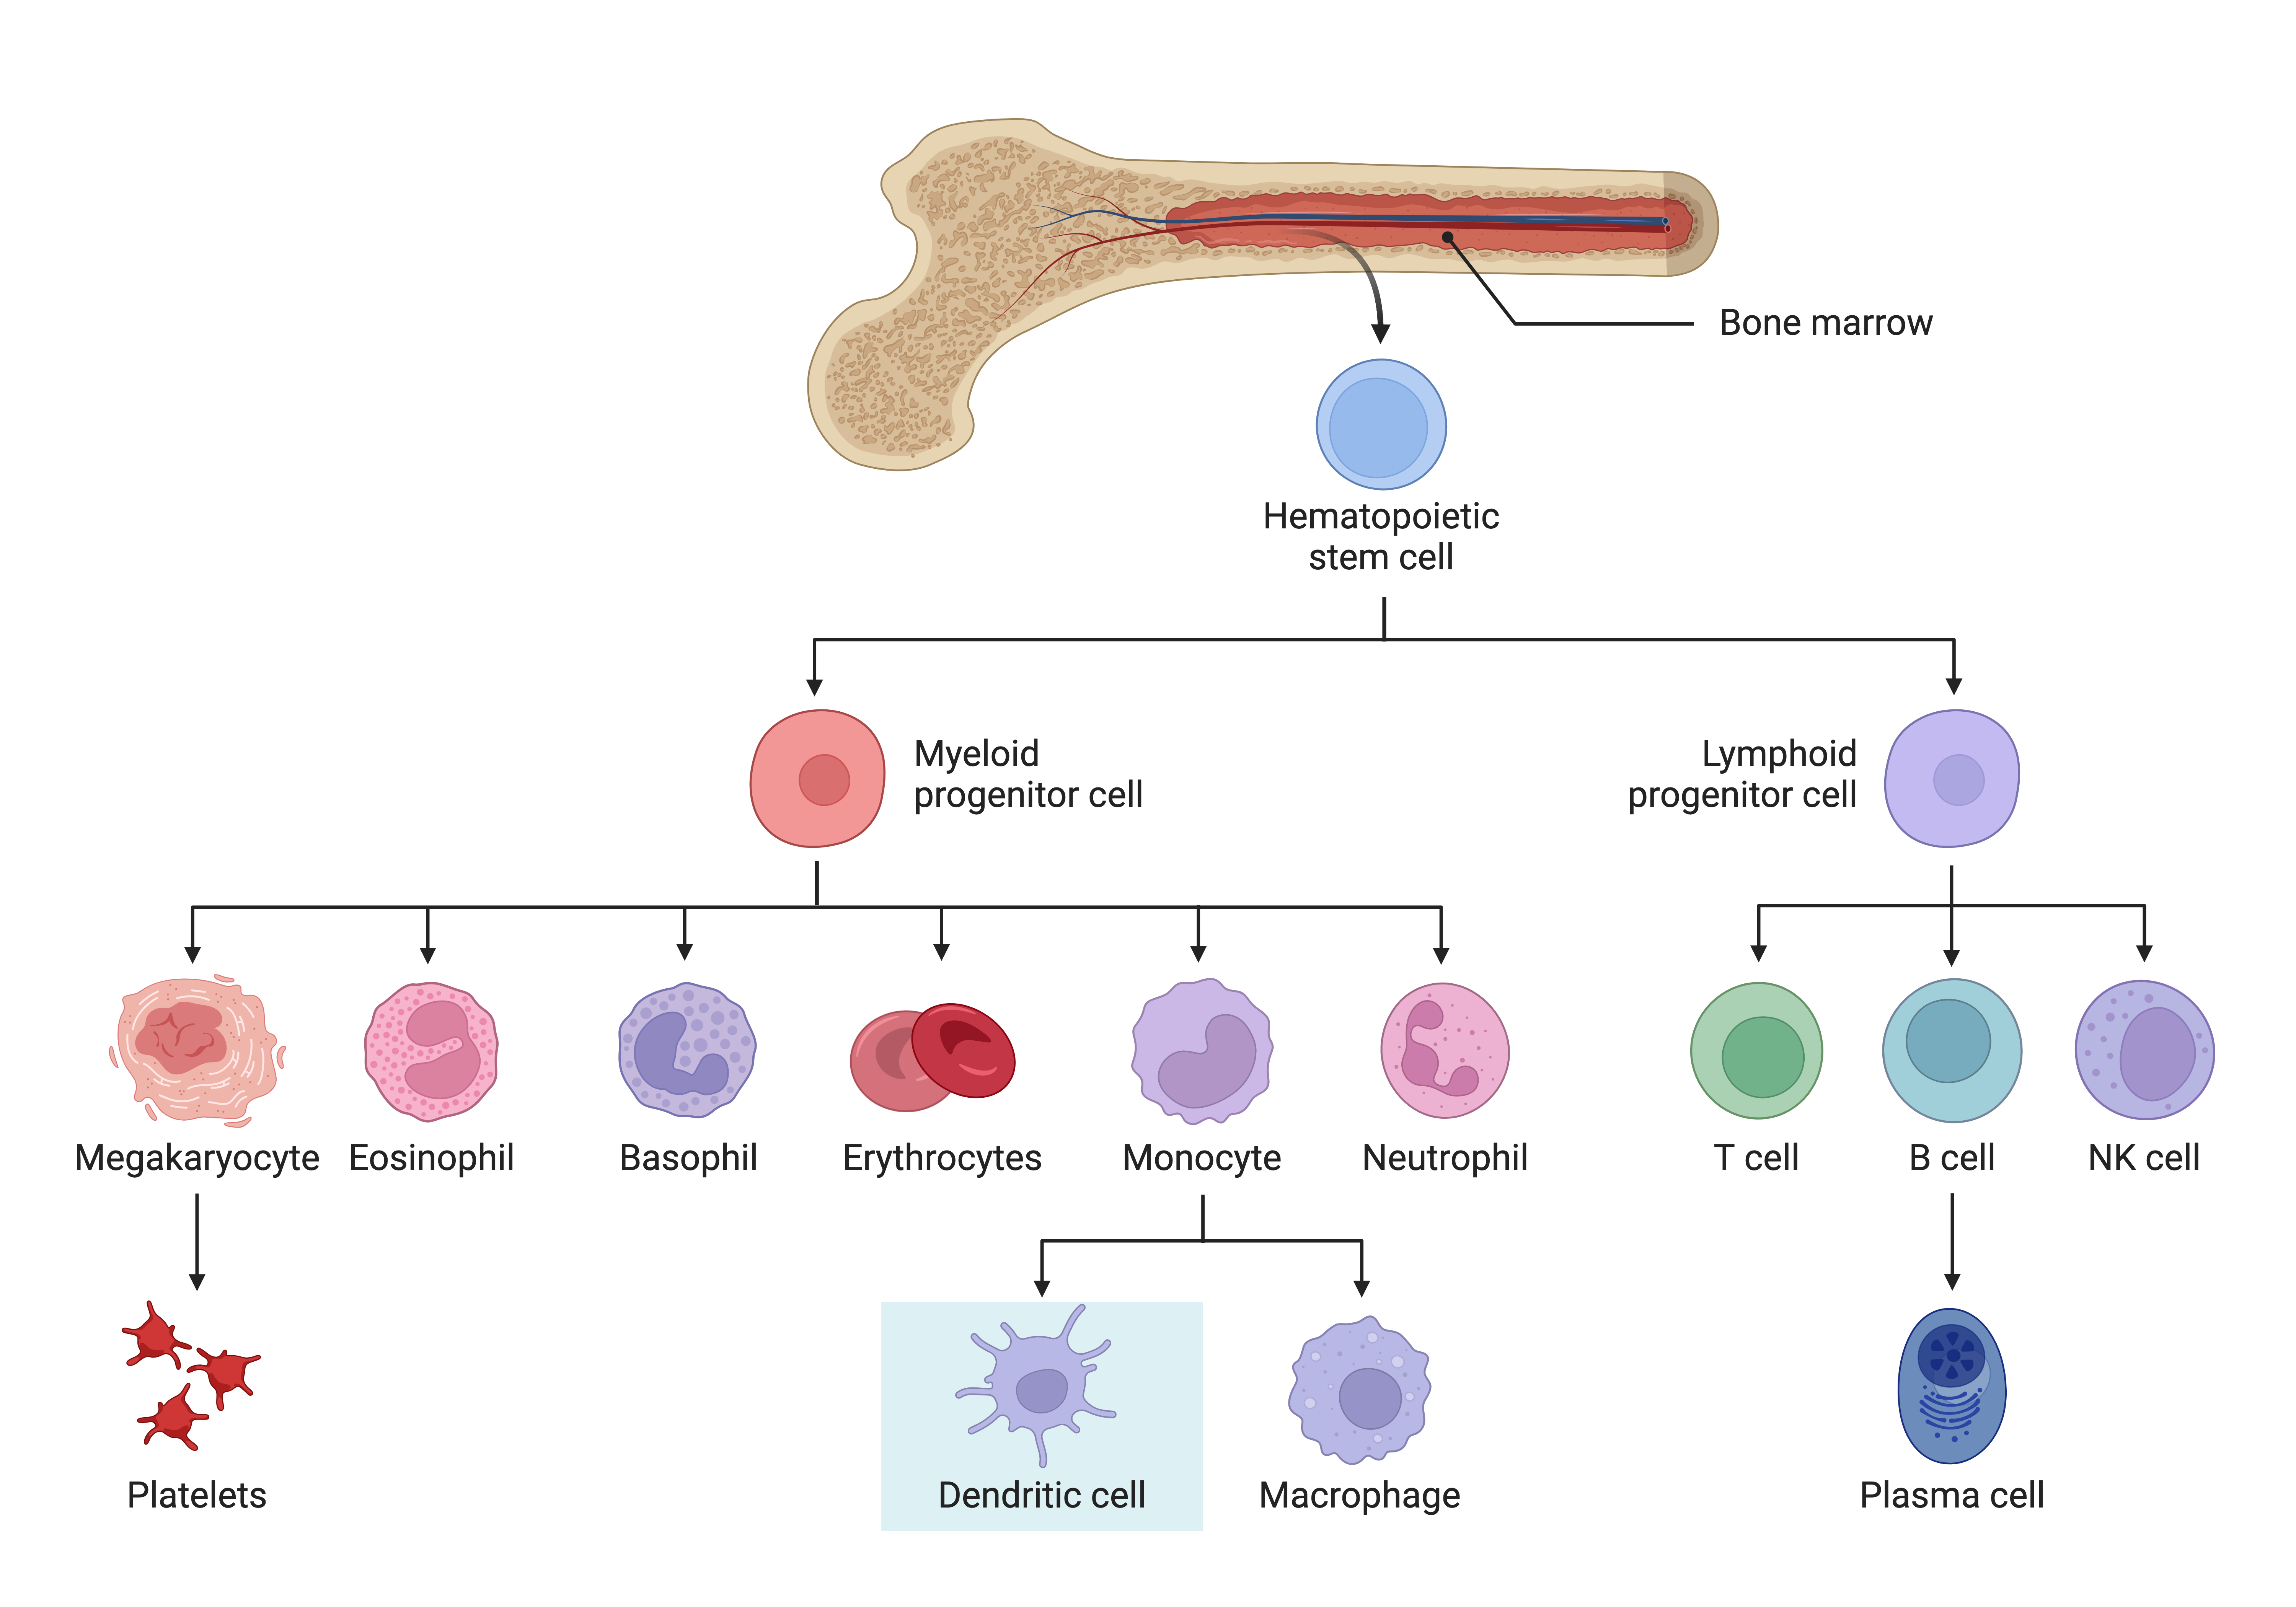
\includegraphics{images/hsc_diff.png}

}

\caption{\label{fig-hsc}Hematopoietic Family Tree Showing how the Mature
Cells in the Various Lineages Are Generated by Self-Generating
Hematopoietic Stem Cells}

\end{figure}%

\subsection{Dendritic Cell Biology}\label{dendritic-cell-biology}

The detection of foreign antigens by DCs represents a crucial stage in
activating the adaptive immune system. Various DC subsets express
diverse sets of pattern recognition receptors (PRRs), allowing for both
overlap and exclusivity in recognizing `danger' signals. The maturation
and activation of DC mediated by PRRs can be gauged by alterations in
the surface expression of costimulatory molecules, changes in the size
and shape of DCs, and the production of different cytokines.

\subsubsection{Overview of Dendritic Cell
Types}\label{overview-of-dendritic-cell-types}

DCs play a crucial role as immune sentinels, essential for initiating
and regulating immune responses. This diverse population exhibits
phenotypic and functional variations in, depending on their location
within the body and their specific immunological functions. In a
non-activated or `steady state', immature DCs continually survey their
local environment, actively seeking foreign antigens for presentation to
T-cells. These immature DCs has elevated expression of CD11c,
intermediate expression of MHC-II, and limited expression of surface
costimulatory molecules such as CD25, CD40, CD69, CD80, CD83, and CD86.
When `steady state' DCs capture antigens, they migrate to lymph nodes to
present the antigens to T-cells. These `mature' DCs exhibit increased
expression of MHCII and costimulatory markers although these DCs may not
be fully activated. Complete activation of DCs relies on their
recognition of `danger signals' that is accomplished through pattern
recognition receptors (PRRs). DCs can be generally classified into three
distinct subsets based on their maturation/activation status:

\begin{enumerate}
\def\labelenumi{\arabic{enumi}.}
\item
  Immature, nonactivated DCs, `steady state' DCs found in the spleen,
  exhibit high levels of CD11c, and low-to-intermediate expression of
  MHC-II and costimulatory markers. In the absence of prior activation,
  these DCs do not generate inflammatory cytokines but can stimulate
  naïve T-cells. Plasmacytoid (p) DCs express lower levels of CD11c and
  MHC-II, are weak stimulators of naïve T-cells, and do not produce
  pro-inflammatory cytokines in the `steady state'.
\item
  Mature but non-activated, and potentially tolerogenic, migratory DCs
  exhibit intermediate CD11c expression and higher levels of MHC-II and
  costimulatory markers on their surface and does not produce
  inflammatory cytokines.
\item
  Mature, activated DCs have encountered `danger signals' in response to
  an invading pathogen or damaged self. Depending on the DC subset these
  DCs produce substantial amounts of inflammatory cytokines very high
  levels of MHC-II and costimulatory molecules on their surface.
\end{enumerate}

DCs recognize pathogen-associated signals through Pattern Recognition
Receptors (PRRs) located on its surface. Since the identification of the
first mammalian Toll-like Receptors (TLRs) that activated the innate
immune system (5), the innate immune system has demonstrated plasticity
in responding to invading pathogens. These activating `danger signals'
recognized by DCs are the following:

\begin{enumerate}
\def\labelenumi{\arabic{enumi}.}
\item
  Pathogen-Associated Molecular Patterns (PAMPs), which are
  evolutionarily conserved molecules associated with pathogens (for
  e.g.~LPS, bacterial and viral nucleic acids), not typically found
  within eukaryotes.
\item
  Damage-Associated Molecular Patterns (DAMPs), such as intracellular
  proteins released by body's own cells undergoing necrosis.
\item
  Inflammatory cytokines.
\end{enumerate}

The response to danger signals triggers alterations in the phenotype and
morphology of DCs. These modifications encompass an augmented expression
of MHC molecules on the cell surface, upregulation of costimulatory
markers, cytokine and chemokine release, and the release of cellular
proteases. Microscopy, flow cytometry analysis, or assays measuring
soluble protein excretion, such as ELISA or Multiplexed Bead-based
Immunoassays, can effectively detect all these changes induced by
maturation or activation.

\subsubsection{Antigen Presentation by Dendritic
Cells}\label{antigen-presentation-by-dendritic-cells}

Immature dendritic cells recognize pathogen-associated molecular
patterns (PAMPs) --- structures that are evolutionarily conserved, such
as microbial LPS, carbohydrates, nucleic acids, and intermediates of
viral replication. This recognition is facilitated through pattern
recognition receptors (PRRs). Various PRRs participate in the innate
recognition of pathogens, including nucleotide-binding
oligomerization-domain (NOD-like) receptors, C-type lectin receptors
(CLRs), Toll-like receptors (TLRs), RIG-I-like helicases, \& active
protein kinase (PKR) (6). Various mechanisms such as macropinocytosis,
endocytosis, and receptor-mediated phagocytosis are employed to capture
foreign antigens after antigen recognition (7--9). Specifically, in the
case of receptor-mediated phagocytosis, it involves the engulfment of
pathogens such as bacterial cells. This process requires actin
re-modeling to create a cup-shaped structure around the foreign
particle, which subsequently closes to form a phagosome. The various
processes of antigen capture by DCs are facilitated by numerous
receptors that transport the antigen to processing compartments (7--9).
DCs convert proteins into peptides, presenting them on major
histocompatibility complex (MHC) molecules, specifically MHC class I and
II (Figure~\ref{fig-dc-present}) (7,8). In the case of lipid antigens,
their processing differs as they are loaded onto non-classical MHC
molecules belonging to the CD1 family (7). Following antigen uptake and
processing, DCs present antigens in the following ways:

\begin{enumerate}
\def\labelenumi{\arabic{enumi}.}
\item
  Via MHC-II to CD4\textsuperscript{+} T lymphocytes (exogenous route):
  This route typically occurs when exogenous peptides are presented by
  DCs through MHC-II molecules. These peptides are derived from proteins
  that have undergone endocytosis and degradation by acid-dependent
  proteases in endosomes (8,10).
\item
  Via MHC-I to CD8\textsuperscript{+} T lymphocytes (endogenous route):
  In this route DCs present intracellular antigens associated through
  MHC class I molecules. For instance, during a viral infection, DCs can
  present viral peptides, allowing the immune system to recognize and
  activate CD8\textsuperscript{+} T lymphocytes, leading to the
  elimination of infected cells (8,10).
\item
  Via cross-presentation: This involves presenting exogenous antigens on
  MHC-I molecules, ultimately stimulating CD8\textsuperscript{+} T
  lymphocytes or cytotoxic T-cells (T\textsubscript{C}cells).
  Phagocytosis is a critical process for cross-presentation, and it is
  noteworthy that this capability is a distinctive feature of DCs,
  particularly specific subsets such as CD8\textsuperscript{+} DCs and
  migratory CD103+ DCs (8,10,11).
\end{enumerate}

\subsection{Dendritic cell isolation and
culture}\label{dendritic-cell-isolation-and-culture}

\subsubsection{Methods for isolating dendritic
cells}\label{methods-for-isolating-dendritic-cells}

DCs makes up only about 0.2 \% of human blood mononuclear cells and can
be isolated and enriched using several methods. One method is to use
density gradient centrifugation over metrizamide to isolate dendritic
cells from human mononuclear cells. Mononuclear cells are isolated from
leukapheresis pack or buffy coat preparation by Ficoll-Paque density
gradient and the T-cells are depleted using magnetic beads conjugated
with anti-TCRα/β monoclonal antibodies. The T-cell depleted cell
suspension is incubated overnight in RPMI1640 media at 37°C on
tissue-culture plates. This allows the monocytes to adhere to the
plastic and helps the DCs to further differentiate into mature DCs in
suspension. The non-adherent T-cells are gently removed, and the process
is repeated a second time to further enrich DCs. The resulting cell
suspension is subjected to gradient centrifugation with sterile 14.5 \%
metrizamide solution. Cells at the interface of the top layer (RPMI1640)
and bottom metrizamide layer are carefully removed which contains 20\%
to 80\% dendritic cells and is largely free of lymphocytes (12,13).
Another method is to isolate adherent monocytes (described above) and
incubate with TNF-α, GM-CSF, and IL-4 for 5-7 days. The differentiation
process occurs withouT-cell proliferation, making the quantity of
monocytes a critical factor for dendritic cell recovery. As monocytes
are more abundant than dendritic cells, this approach can lead to higher
yields compared to the previous protocol (14). Highly purified dendritic
cell preparations can be obtained from these populations by a process
known as magnetic-activated cell sorting (MACS). In this protocol
mononuclear cells are incubated with a mix of anti-CD3, -CD14, -CD19,
and -CD56 monoclonal antibodies conjugated with magnetic beads. Using a
magnetic separation apparatus lymphocytes, monocytes, and NK cells are
depleted and the resulting cell suspension is incubated overnight in
RPMI1640 media at 37°C on tissue-culture plates. The non-adherent
T-cells are gently removed and incubated with anti-CD83 antibody
conjugated to magnetic beads. The resulting CD83 positive population
contains highly enriched population of DCs for various downstream
applications (12,13).

\begin{figure}

\centering{

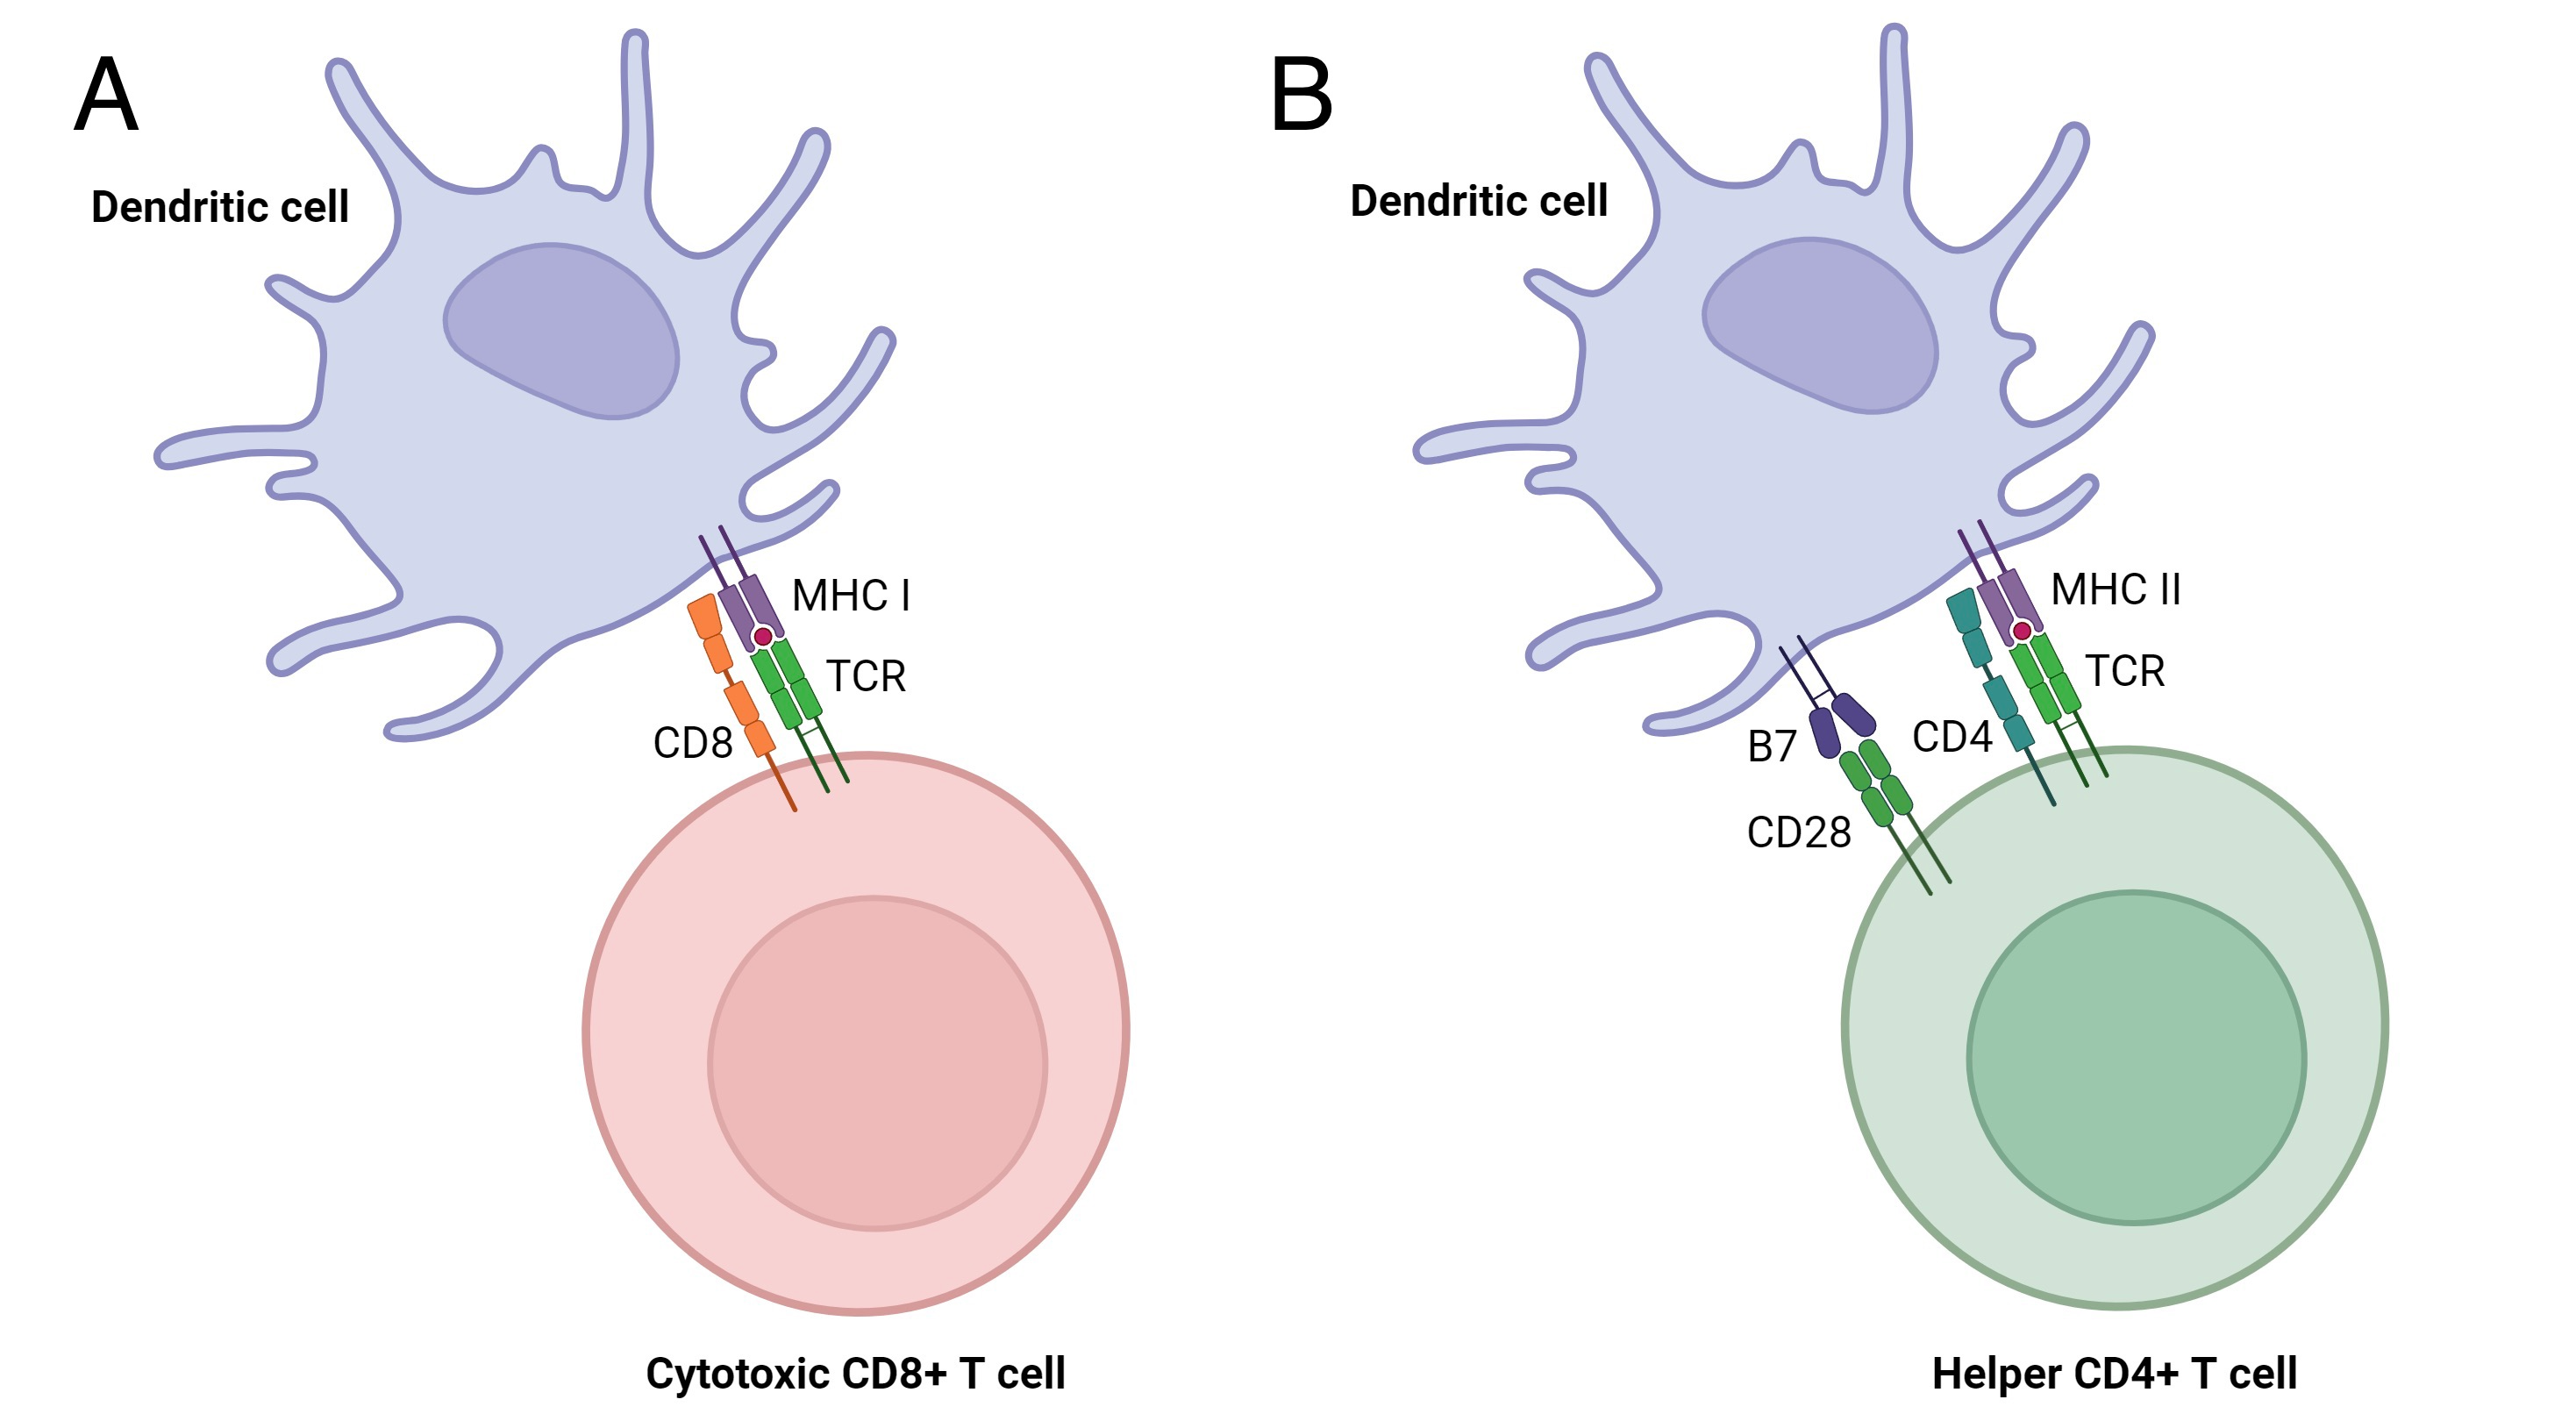
\includegraphics{images/fig_2.png}

}

\caption{\label{fig-dc-present}An illustraion showing dendritic cells
presenting antigens to both MHC Class-I (A) and -II (B) molecules on
T-cells.}

\end{figure}%

\subsubsection{Maturation of dendritic
cells}\label{maturation-of-dendritic-cells}

DC maturation is a crucial step that should ideally precede vaccination.
However, there is currently no consensus on the most suitable methods to
generate robust immunostimulatory DCs. Various combinations of
maturation stimuli have been explored, including proinflammatory
cytokines, CD40L/ CD154), and Toll-like receptor agonists (15--17). The
utilization of Toll-like receptor agonists leads to elevated IL-12
levels, resulting in a potent activation of DCs and subsequent effective
immune activation. The maturation process is pivotal for efficient
vaccine production because mature DCs generally exhibit enhanced
expression of co-stimulatory molecules and increased production of
cytokines and chemokines. In contrast, immature DCs lack the ability to
induce antigen-specific responses and may potentially foster the
differentiation of regulatory T-cells.

\subsubsection{Optimization of dendritic cell
yield}\label{optimization-of-dendritic-cell-yield}

In order to increase DC yield it is crucial to start with large volume
of human blood mononuclear cells. Small blood volumes are inadequate for
dendritic cell isolation. When dealing with limited blood volumes it is
recommended to generate dendritic cells from monocytes. Freshly isolated
mononuclear cells are ideal, but satisfactory results can be achieved
using 24 hour old blood preparations stored on ice. Leukocyte-enriched
`leukopaks' obtained within the last 24 hours can provide a significant
number of mononuclear cells, typically ranging from 2 - 12 ×
10\textsuperscript{8} cells per leukopak. Alternatively, `buffy coats'
from donated blood units can be used. Care must be taken with isolation
procedures, as it may affect neutrophils within leukopaks, making it
difficult to remove neutrophils which eventually will impact DC purity.
A critical step of DC isolation is the removal of non-adherent T-cells.
The tissue culture plate must be washed throughly with warm media using
a pipette with sufficient force to remove non-adherent T-cells. The cell
morphology can be roughly assessed through phase-contrast microscopy.
DCs are large and irregular shaped with long membrane processes and can
be easily identified (Figure~\ref{fig-dc}). For higher dendritic cell
purity, two metrizamide density gradient centrifugation steps can be
performed. Contaminating B lymphocytes and monocytes can be further
depleted through adherence to Ig-coated plates. Lineage-associated
monoclonal antibodies (mAbs) can also be employed for depletion using
magnetic beads or panning. Depleting contaminating cells through
F\textsubscript{C} receptor-mediated procedures is effective but may
limit dendritic cell heterogeneity, considering dendritic cells express
CD32 and CD64 F\textsubscript{C} receptors (18).

\subsection{Antigen Loading onto Dendritic
Cells}\label{antigen-loading-onto-dendritic-cells}

\subsubsection{Techniques for Loading Antigens onto Dendritic
Cells}\label{techniques-for-loading-antigens-onto-dendritic-cells}

Loading DCs with peptides, tumor cells, or intact proteins represents
the most common method, typically conducted prior to maturation
(Figure~\ref{fig-dc-loading}). In this approach, peptides are directly
loaded on either MHC-I or MHC-II molecules on the surface of the DCs.
Conversely, tumor cells or intact proteins need to be processed and
presented by the DCs to activate CD4\textsuperscript{+} and
CD8\textsuperscript{+} T-cells. The primary drawback associated with
peptide usage is the requirement to identify the patient's haplotype and
the specific peptides that would bind to these particular haplotypes.
Contrastingly, utilizing tumor cells or intact proteins is advantageous
as it is not restricted to particular haplotypes (15,19,20).

\begin{figure}

\centering{

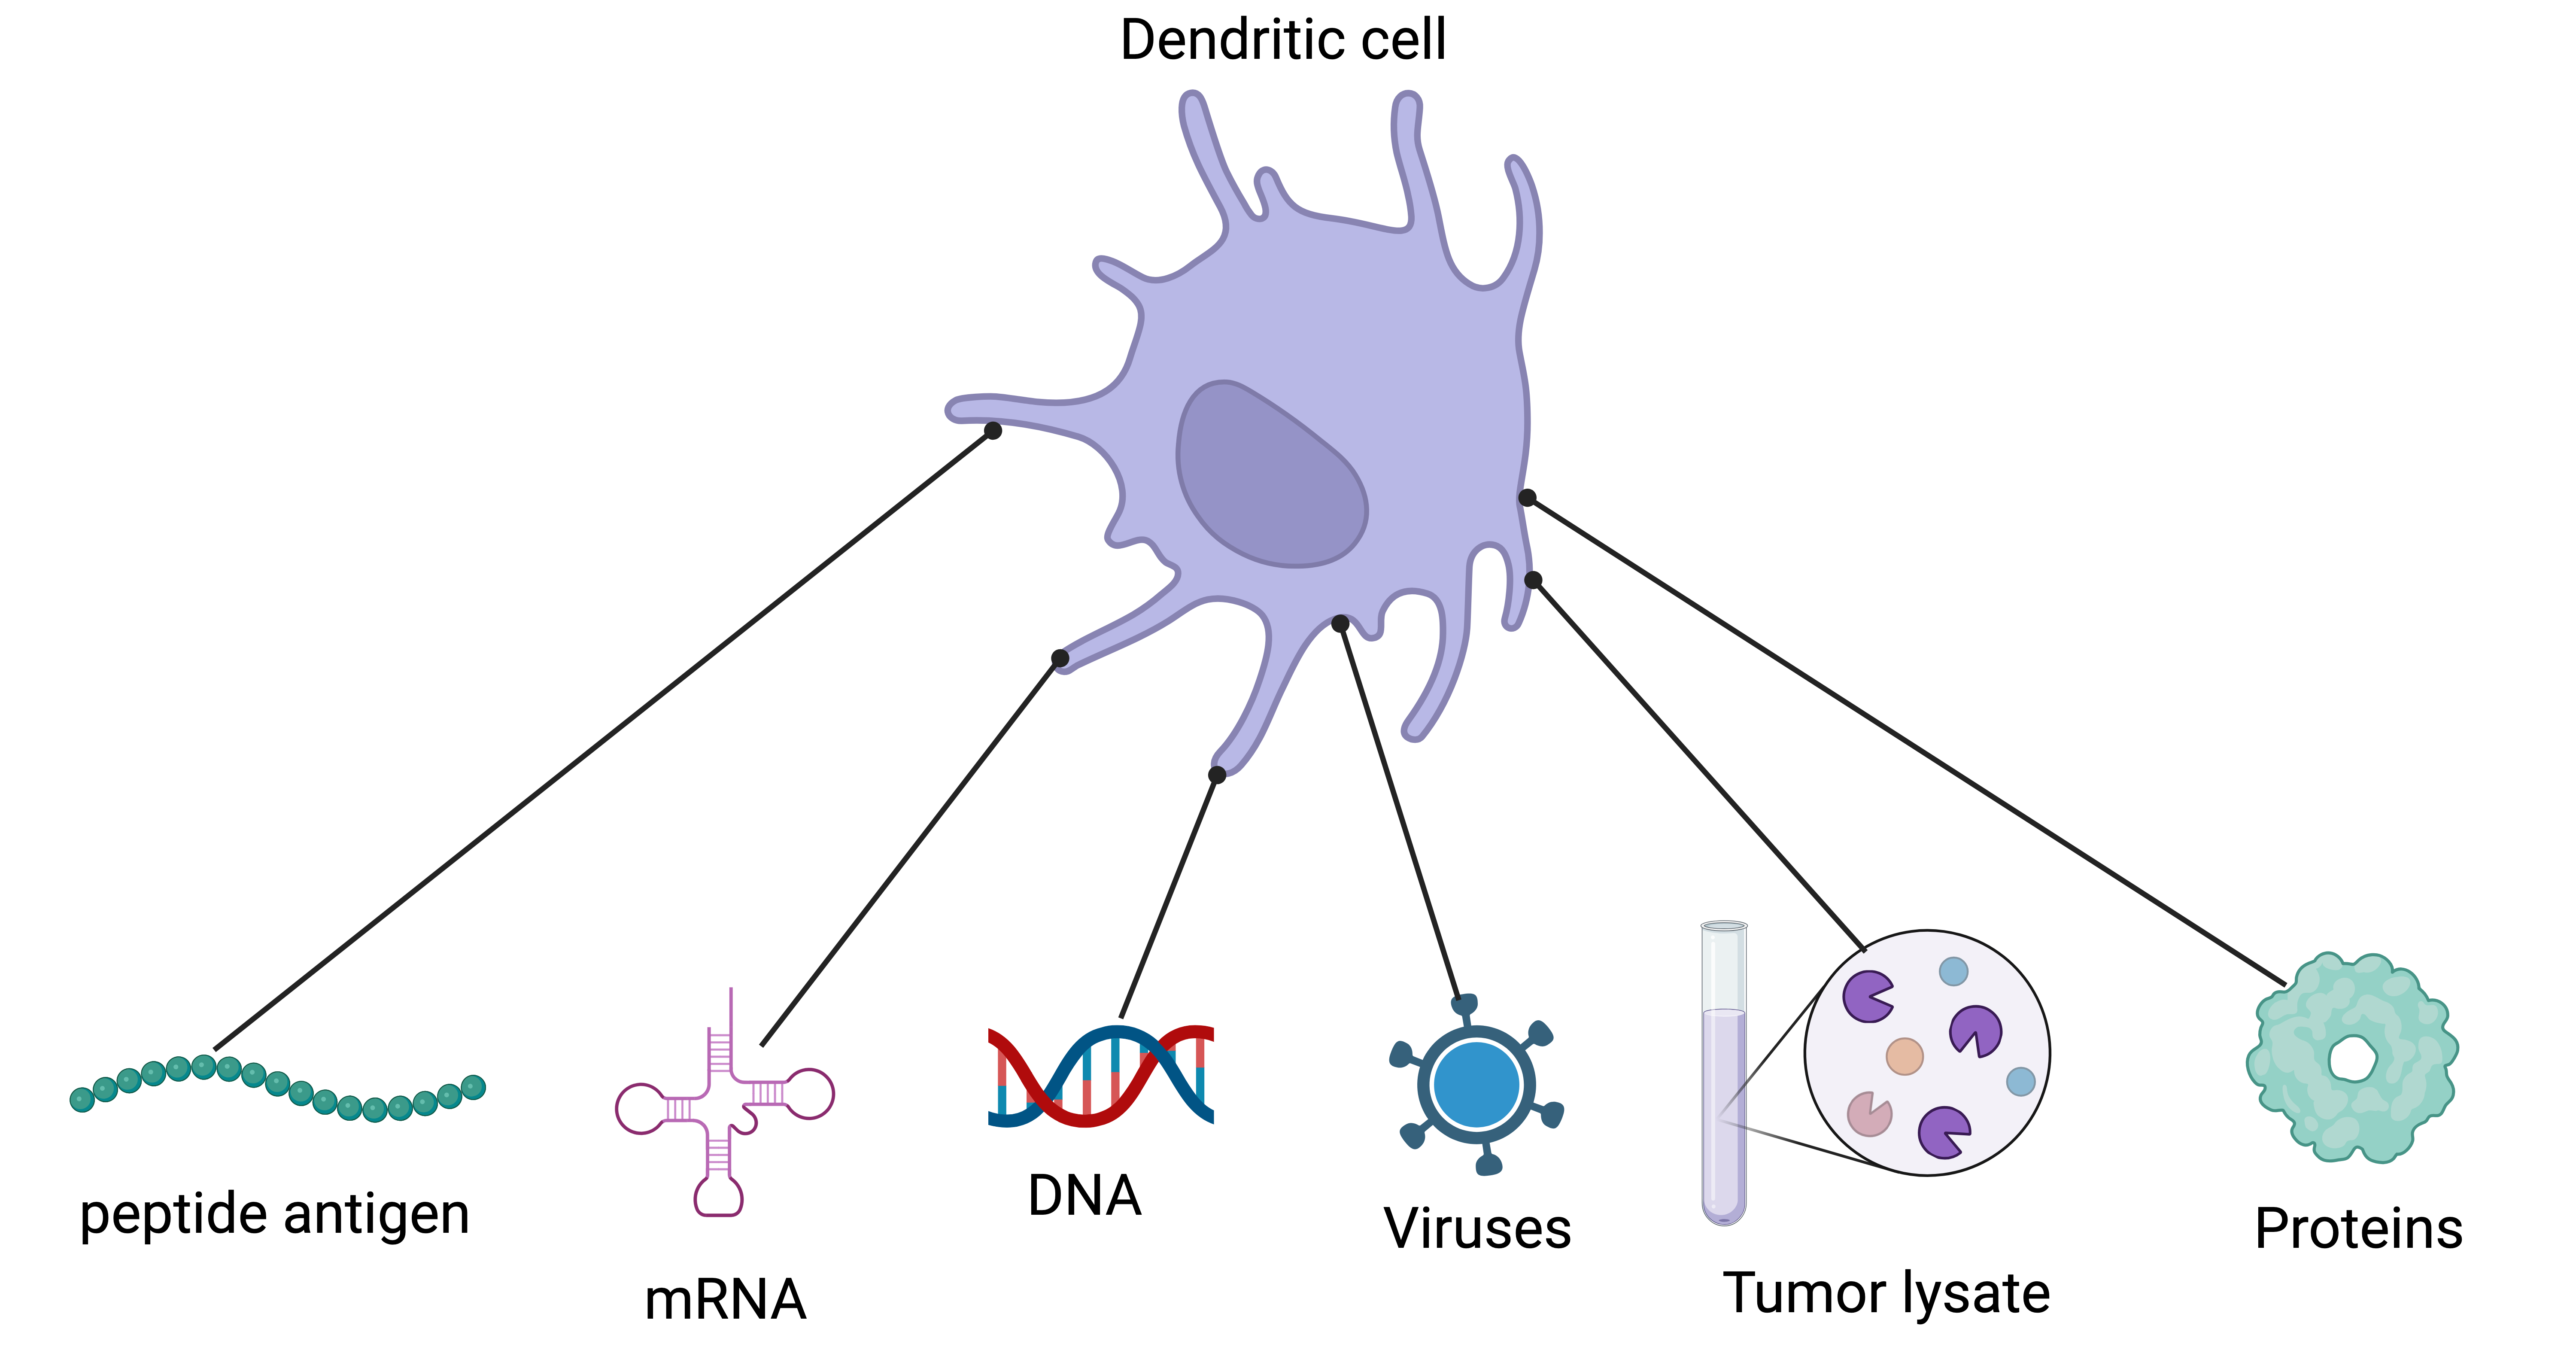
\includegraphics{images/ag_loading.png}

}

\caption{\label{fig-dc-loading}Distinct DC vaccine loading approaches
have been tested in clinical trials: loading of DCs with peptides,
proteins, and tumor lysates; mRNA transfection; and delivery of DNA and
the use of viral vectors.}

\end{figure}%

The use of viral vectors presents an appealing alternative for loading
antigenic material onto dendritic cells (DCs), as it enables gene
insertion encoding tumor antigens or intact proteins, while allowing for
the removal of virulence or replication factor genes. In some instances,
the vector itself may promote DC maturation, eliminating the need for an
additional maturation process. Another advantage lies in the ability to
incorporate genes encoding co-stimulatory cytokines, thereby enhancing
DC immunogenicity. However, the existence of pre-existing immunity
against the viral vector might diminish the patients' capacity to induce
\emph{in vivo} responses, that maks safety a major concern.
Lentivirus-based vectors has been shown to be significantly less
immunogenic due to the removal of the viral protein encoding genes.
Additionally, lentivirus-based vectors offer specific advantages,
including the potential to activate the innate immune system through
cytoplasmic or endosomal molecules such as TLRs, RIG-I, and PKR
(15,21--24).

An alternative and appealing approach involves loading DCs with
messenger RNA (mRNA) which encodes tumor-associated antigens (TAAs), a
method proven to elicit CD4\textsuperscript{+} and
CD8\textsuperscript{+} T-cell responses. These mRNAs, characterized by a
short half-life and not integrated into the host genome, can be directly
loaded onto DCs without the need for viral vectors or knowledge of the
patient's haplotypes (6,15). Furthermore, mRNA transfection allows for
the presentation of several antigenic epitopes, along with loading
options involving maturation stimuli (such as CD40L) or cytokines.
Electroporation has been identified as the most efficient method for
introducing mRNA into DCs without the requirement for additional
reagents (15,25--27).

\subsubsection{Enhancing Antigen Presentation
Efficiency}\label{enhancing-antigen-presentation-efficiency}

Dendritic cells (DCs), acting as vigilant sentinels in tissues,
continuously survey their local environment, capturing antigens for
presentation to CD4\textsuperscript{+} T\textsubscript{H}cells or
CD8\textsuperscript{+} T\textsubscript{C}cells on MHC-I or MHC-II
molecules, respectively (28,29). The uptake of exogenous antigen is
accomplished through various mechanisms, including phagocytosis (30,31),
receptor-mediated endocytosis (32--34), or micropinocytosis (35,36),
depending on the DC subtype and activation state (32). For instance,
Langerhans cells (LC) and CX3CR1\textsuperscript{+} macrophages at
barrier sites like the intestinal epithelium (37,38) utilize dendritic
projections to sample antigens. Dermal cDC2 can access epicutaneously
applied antigen through hair follicles (39). Following antigen uptake,
human LC migrate through the dermis and then to skin-draining lymph
nodes (skin-dLNs) in a CXCR4-dependent manner, subsequently transferring
antigen-MHC-II complexes to dermal cDC through direct contact or
indirectly within the dermis (40). This transfer mechanism potentially
enhances the efficiency of antigen transport to the LN, as dermal cDCs
migrate faster and disperse more widely within the LN than LCs.

cDC2, with a notable proficiency for antigen uptake in the skin,
constitute the majority of antigen-positive cells in skin-dLNs following
the administration of particulate antigen (41,42). They also play a
crucial role in capturing tumor antigens and transporting them to LNs
for T-cell presentation (43). Soluble and particulate antigens below 70
kDa can reach LNs without active cellular transport, relying on a
conduit network (44,45). Nevertheless, cDC2 show a higher capacity for
the uptake of soluble antigen per cell and are overrepresented among
antigen-positive cells in various settings, indicating an intrinsic
capability for exogenous antigen uptake (46,47). Their optimal
positioning within tissues, especially in proximity to lymph-borne
antigens near the subcapsular sinus in LNs, further supports their
efficient antigen capture (42,46).

In contrast, cDC1, situated deep within the LN paracortex (46), excel at
capturing cell-associated antigens and dead cells through specific
receptors like Clec9A, DEC205, Axl, and TIM3 (48). This subtype
predominantly processes cell-associated antigens via cross-presentation
on MHC-I, crucial for antiviral and antitumor immunity (48). Monoclonal
antibodies targeting receptors such as CLEC9a and DEC205 have
successfully enhanced antigen uptake and cross-presentation in
vaccination contexts (49--51). Additionally, both monocyte-derived DCs
(moDC) and cDC2 can engage in cross-presentation, indicating a degree of
redundancy in this pathway, particularly notable in humans (52--54).

DCs constitute the primary population of antigen-presenting cells
\emph{in vivo}, playing a crucial role in initiating antigen-specific
activation and expansion of naive CD4\textsuperscript{+} T-cells through
interactions involving peptide--MHC-II binding with the TCR and
co-stimulatory signaling (49,55). Among DC subtypes, cDC2 stands out for
its remarkable efficiency in processing exogenous antigens for
presentation on MHC-II, resulting in superior CD4\textsuperscript{+}
T-cell proliferation compared to cDC1. This specialization is believed
to be influenced by the expression of Irf4 in cDC2, as IRF4 has been
linked to enhanced peptide--MHC-II complex formation in these cells
(55).

Beyond facilitating CD4\textsuperscript{+} T-cell activation and
proliferation, the communication between DCs and CD4\textsuperscript{+}
T-cells during antigen presentation plays a crucial role in determining
the differentiation fate of T helper (T\textsubscript{H}) cells. Several
factors, including the strength and duration of co-stimulatory signals
and interactions between peptide-MHC-II and TCR, are implicated in
regulating the T\textsubscript{H} cell differentiation program (56).

\subsection{Strategies for Dendritic Cell
Activation}\label{strategies-for-dendritic-cell-activation}

\subsubsection{Use of Adjuvants in Dendritic Cell
Activation}\label{use-of-adjuvants-in-dendritic-cell-activation}

An effective adjuvant should be designed to specifically target DCs to
enhance antigen presentation and activate immune responses. DCs, a type
of white blood cell, are highly proficient in capturing, processing, and
presenting antigens to T-cells. When appropriately activated, DCs engage
with CD4\textsuperscript{+} T lymphocytes through surface receptors like
MHC-II, CD80, and/or CD86, and they release cytokines such as IL-12,
initiating T-cell activation.

In mice, DCs are identified by the expression of CD11c and can be
categorized into broad populations based on CD8a and CD4 expression,
resulting in CD8a\textsuperscript{+}, CD4\textsuperscript{+}, and
double-negative (DN) DCs (CD8a\textsuperscript{-}CD4\textsuperscript{-})
subsets (57,58). Conversely, in humans, DC subpopulations are not
differentiated by CD4 and CD8 expression. DCs also express pattern
recognition molecules, specifically Toll-like receptors (TLRs), that act
as activation signals. The TLR family comprises 11 members (TLR1--11)
that recognize several PAMPs (59), inducing the maturation and migration
of DCs to lymph nodes which in turn promote immune responses. While TLR2
and TLR4 mRNAs are present in all murine DC subsets (60), the expression
of TLR9 protein have also been demonstrated (61,62). TLR2 is notable for
recognizing a broad range of lipid ligands derived from different
microbe types, including bacteria. It forms heterodimers with either
TLR6 or TLR1 for recognizing di- acylated or tri-acylated lipids,
respectively. However, it is suggested that TLR2 may also function as
homodimers for signaling, as seen in the recognition of synthetic
lipopeptides.

\subsubsection{Cytokine-Based Activation
Methods}\label{cytokine-based-activation-methods}

A novel approach to antigen loading involves the direct antigen
targeting to dendritic cells (DCs) \emph{in vivo}, aiming to promote
anti-tumorigenic immune responses (64). This strategy presents a
promising option for DC immunotherapy, bypassing the costly and
labor-intensive \emph{ex vivo} DC generation process. It allows to
produce vaccines on a larger scale, eliminating the need for customized
vaccines for each patient.

Early methods for \emph{in vivo} DC targeting included engineering
irradiated tumor cells to secrete granulocyte-macrophage
colony-stimulating factor (GM-CSF) (65). GM-CSF was employed to recruit
and promote the function of antigen-presenting cells (APCs). The
strategies employed included the use of autologous tumor cells modified
to produce GM-CSF via gene transfer mediated by retroviruses or
adenoviruses, allogeneic tumor cell lines that had been genetically
altered to continuously produce GM-CSF, or a combination of autologous
tumor cells with cell lines that secrete GM-CSF. Clinical studies
utilizing these techniques have shown they can attract dendritic cells,
granulocytes, macrophages, and T-cells to the site of vaccination.
Typically, patients exhibited delayed-type hypersensitivity responses
that involved CD4\textsuperscript{+} and CD8\textsuperscript{+} T-cells,
eosinophils, and macrophages following the vaccinations (66--68).
Examination of tumor samples from individuals who received the vaccine
showed significant tumor cell death and infiltration by cytotoxic
CD4\textsuperscript{+} and CD8\textsuperscript{+} T-cells and plasma
cells, which produced strong cytokine responses upon reactivation,
demonstrating the effective generation of immune responses specific to
the tumor.

Extended GM-CSF production within the tumor environment is linked to
disease progression in some experimental conditions, including a Phase
III study that tested the immunization with irradiated GM-CSF-producing
allogeneic prostate cancer cells in patients with metastatic disease
resistant to hormone therapy (65). This advancement could be due to the
immune system becoming tolerant because of long-term administration of
GM-CSF, which could lead to the recruitment of myeloid suppressor cells
or cause myeloid precursors to develop into immature, tolerogenic
dendritic cells (69,70).

Newer strategies are being developed that aim at dendritic cell-specific
molecules, such as Fc receptors, CD40, and C-type lectin receptors
(CLRs). CLRs are of particular interest because they are expressed
differently across DC subsets and include DEC205, DC-SIGN, mannose
receptor (MR), and Dectin-1. These receptors play a crucial role in the
identification and capture of glycosylated self-antigens and pathogens
for antigen presentation, as well as in the movement of DCs,
interactions between DCs and T-cells, and the activation of subsequent
immune responses (70). Initial experiments that targeted antigens to
DCIR2 and DEC205 found that without activating signals for DCs, immune
tolerance was induced, while the simultaneous administration of
DC-activating signals was required to trigger immune responses (34).
Later experiments that targeted antigens to various CLRs along with a
DC-activating signal were successful in eliciting strong
CD4\textsuperscript{+} and CD8\textsuperscript{+} T-cell responses
(51,71). Additionally, directing antigens towards CLRs has been shown to
improve antibody responses (72). While most of this research has been
conducted in mice, there are emerging studies in humans focusing on MR
(73) and DC-SIGN (74), showing promising results in the activation of
naive and memory tumor-specific T-cell responses. Nevertheless, further
research is necessary to adapt this promising approach for clinical use
in humans.

\subsubsection{Genetic Modification for Enhanced
Functionality}\label{genetic-modification-for-enhanced-functionality}

Although there is knowledge about signals for dendritic cell (DC)
maturation and activation, the optimal signal to activate T-cells
\emph{in vivo} remain unclear. Current clinical trials of cancer
immunotherapy use DCs from various sources, including those isolated
directly from unmobilized or Flt3 ligand-mobilized peripheral blood, or
generated \emph{in vitro} from CD34\textsuperscript{+} progenitors,
CD14\textsuperscript{+} monocytes, or adherent peripheral blood
mononuclear cells. Immature DCs are loaded with antigens in various
forms, such as peptides, proteins, tumor lysates, apoptotic bodies, or
tumor cell fusions (Figure~\ref{fig-dc-loading}). Gene transfer through
DNA or messenger RNA encoding the antigen has also been investigated for
antigen loading and processing. These loaded DCs may undergo further
processing by maturation with second signals like tumor necrosis
factor-α, CD40 ligand, or monocyte-conditioned media before
administration to patients via different routes, such as intravenous,
intradermal, subcutaneous, or direct intralymphatic or intranodal
injection.

Mature DCs within secondary lymphoid organs express high levels of
costimulatory molecules, facilitating antigen presentation. However,
several issues persist regarding gene modification of DCs. These include
questions about uniform maturation, persistence of molecule expression,
the potential for enhanced function with higher levels of expression,
and the broader impact of genetic modification on DC function. Studies
suggest that using exogenous expression systems like viral vectors
engineered to express crucial molecules can optimize the delivery and
processing of antigens. One study demonstrates the effectiveness of
their strategy for modifying DCs and improving their \emph{in vitro}
performance (75). However, uncertainties remain, including the optimal
strategy for gene expression or repression, concerns about the viral
vector system's potential impact on DC functions, and questions about
the efficiency of migration for matured DCs and whether fully matured
DCs should be administered directly or matured \emph{in vivo}. Despite
these uncertainties, Hodge et al.'s experiments show that DC function
can be manipulated through genetic modification, paving the way for
further exploration of their biologic activity and role in eliciting
authentic antitumor responses in patients.

\subsection{Dendritic Cell Vaccines
Design}\label{dendritic-cell-vaccines-design}

In recent years, there has been clinical promise in reprogramming the
immune system against cancer. Dendritic cells (DCs) emerge as a
compelling target for immunotherapy due to their capacity to capture and
present tumor-associated antigens (TAAs) through various mechanisms,
thereby initiating robust effector responses against the tumor (76--78).
Beyond direct antigen presentation, other intrinsic properties of DCs
play a crucial role in immunotherapy. These include their ability to
migrate between lymphoid and non-lymphoid tissues, regulate cytokine and
chemokine gradients, and control inflammation which are essential for
achieving systemic and enduring anti-tumor effects. Personalized
vaccines involving patient-derived DCs manipulated \emph{ex vivo} have
been extensively investigated to harness these features. Typically,
these therapies are developed by isolating hematopoietic stem and
progenitor cells or monocytes from peripheral blood. These cells undergo
treatment with recombinant cytokines to induce differentiation, are
stimulated for maturation, and are loaded with TAAs in various forms.
This comprehensive process has been employed in numerous preclinical and
clinical studies (79).

\subsubsection{Design, Manufacturing and Quality Control of Dendritic
Cell
Vaccines}\label{design-manufacturing-and-quality-control-of-dendritic-cell-vaccines}

The treatment landscape for various malignant diseases is evolving, with
tumor vaccines gaining prominence in therapeutic strategies. The
effectiveness of these innovative products is being rigorously evaluated
through numerous global clinical trials ((80)). Cell-based vaccines in
the European Union must align with a specified definition. According to
this definition, somatic cell therapy involves the use of autologous
(patient-derived), allogeneic (from a different human subject), or
xenogeneic (originating in animals) cells whose characteristics have
been significantly modified (81). Somatic cell therapy medicinal
products encompass cells that are genetically modified, unless the
genetic modification is unrelated to therapeutic, diagnostic, or
preventive objectives, as is the case with primary tumor cells
immortalized through gene transfer (81).

Currently, tumor vaccines are not covered by the European Pharmacopoeia,
and specific guidelines are lacking for both tumor and therapeutic
vaccines. Good manufacturing practice (GMP) principles should me adhered
to during manufacturing of cell-based tumor vaccines in the EU. The EU
is also preparing guidelines for GMP inspections of gene-therapy and
vaccine products (European Medicines Agency, 2021). The European
Medicines Agency published a ``points to consider'' document on the
manufacture and quality control of somatic cell therapy products, which
may be subject to modification in the future to incorporate emerging
technologies like tissue engineering (European Medicines Agency, 2001).
This document also addresses genetic manipulation of cells and should be
read alongside the guidance on the quality, preclinical, and clinical
aspects of gene-transfer medicinal products, which deals with specific
issues related to gene transfer methodologies involving plasmids or
viruses and addresses safety concerns associated with certain
gene-transfer approaches (European Medicines Agency, 2001).

\subsubsection{Challenges and
Limitations}\label{challenges-and-limitations}

Dendritic cells (DCs) are typically found in an immature state in
circulation and peripheral tissues. Upon receiving maturation signals,
they undergo changes such as upregulation of chemokine receptors,
increased surface expression of MHC molecules, and upregulation of
costimulatory models. These changes facilitate their migration to lymph
nodes, enhance antigen presentation, and amplify T-cell responses. The
type of maturation signals determines the phenotypes of DCs, influencing
their interactions with T-cells and the cytokines they secrete (82).
While DCs play a crucial role in activating the immune system, they can
also induce immune tolerance, potentially hindering effective vaccine
strategies. Studies have linked immature DCs to the promotion of
regulatory T-cell development, contributing to peripheral
self-tolerance. In some cases, immature DCs induced nonproliferative
responses and IL-10 secretion, characteristic of a Treg population. The
use of antigen-pulsed immature DCs has even led to antigen-specific
immune suppression, inhibiting pre-existing antigen-specific T-cell
function (83). To address these challenges, vaccines need to incorporate
signals that ensure full maturation and activation of DCs before
administration. Attempts to exploit immature DCs to promote anergy have
been made in transplantation and autoimmunity settings. However, in
cancer vaccines, ensuring full maturation and appropriate activation of
DCs is crucial to overcome immune tolerance barriers. Researchers have
also demonstrated that inappropriately activated DCs, even with mature
features, can induce T-cell tolerance. Understanding the signals that
lead to tolerogenic DC states is essential for directing the choice of
maturation signals and targeting factors present in the tumor
microenvironment that mediate tolerance. Moreover, maturation alone may
not be sufficient for immune activation, as demonstrated in studies
where mature DCs led to the expansion of T\textsubscript{REG}
populations in myeloma patients. Confirming DC maturity and phenotype
through cell-surface markers and cytokine secretion before vaccine
administration is crucial for cancer vaccines to overcome the challenge
of immune tolerance (84).

\subsection{Clinical Trials and
Outcomes}\label{clinical-trials-and-outcomes}

Effective cancer vaccines can function as preventive agents against
cancers linked to infectious diseases, such as hepatitis B virus or
human papillomavirus, and serve as onco-therapeutic agents. The latter
approach relies on the recognition of specific tumor-associated antigens
(TAAs) by CD3\textsuperscript{+} T-cells within the host body.
Vaccination can enhance the existing immune response against TAAs or
induce a \emph{de novo} response. Dendritic cells (DCs), known for their
effectiveness as antigen-presenting cells (APCs), play a crucial role in
both major histocompatibility complex class I (MHC-I) and II (MHC-II)
presentation to CD8\textsuperscript{+} and CD4\textsuperscript{+}
T-cells, respectively. Dendritic cells exhibit migratory capabilities
between lymphoid and non-lymphoid tissues, modulating cytokine and
chemokine gradients to regulate inflammation and lymphocyte homing.

\begin{longtable}[]{@{}
  >{\raggedright\arraybackslash}p{(\columnwidth - 6\tabcolsep) * \real{0.2329}}
  >{\raggedright\arraybackslash}p{(\columnwidth - 6\tabcolsep) * \real{0.2329}}
  >{\raggedright\arraybackslash}p{(\columnwidth - 6\tabcolsep) * \real{0.2329}}
  >{\raggedright\arraybackslash}p{(\columnwidth - 6\tabcolsep) * \real{0.3014}}@{}}
\caption{Overview of clinical trials registered on
\href{https://www.clinicaltrials.gov/}{clinicaltrials.gov} between
January 2022 and October 2024 testing dendritic cell-based immunotherapy
in cancer patients.}\label{tbl-clin}\tabularnewline
\toprule\noalign{}
\begin{minipage}[b]{\linewidth}\raggedright
NCT Number
\end{minipage} & \begin{minipage}[b]{\linewidth}\raggedright
Study Status
\end{minipage} & \begin{minipage}[b]{\linewidth}\raggedright
Conditions
\end{minipage} & \begin{minipage}[b]{\linewidth}\raggedright
Combinatorial Treatment
\end{minipage} \\
\midrule\noalign{}
\endfirsthead
\toprule\noalign{}
\begin{minipage}[b]{\linewidth}\raggedright
NCT Number
\end{minipage} & \begin{minipage}[b]{\linewidth}\raggedright
Study Status
\end{minipage} & \begin{minipage}[b]{\linewidth}\raggedright
Conditions
\end{minipage} & \begin{minipage}[b]{\linewidth}\raggedright
Combinatorial Treatment
\end{minipage} \\
\midrule\noalign{}
\endhead
\bottomrule\noalign{}
\endlastfoot
\href{https://clinicaltrials.gov/study/NCT05809752}{NCT05809752} &
Recruiting & Triple Negative Breast Cancer & Single agent \\
\href{https://clinicaltrials.gov/study/NCT06435910}{NCT06435910} &
Recruiting & Multiple Myeloma & Single agent \\
\href{https://clinicaltrials.gov/study/NCT05504707}{NCT05504707} &
Recruiting & Triple Negative Breast Cancer & Single agent \\
\href{https://clinicaltrials.gov/study/NCT04912765}{NCT04912765} &
Recruiting & Hepatocellular Carcinoma & Nivolumab \\
\href{https://clinicaltrials.gov/study/NCT06253234}{NCT06253234} &
Recruiting & WHO Grade III/IV Gliomas & Single agent \\
\href{https://clinicaltrials.gov/study/NCT05773859}{NCT05773859} &
Recruiting & Ovarian Carcinoma & Single agent \\
\href{https://clinicaltrials.gov/study/NCT05767684}{NCT05767684} &
Recruiting & Solid Tumor & Nivolumab \\
\href{https://clinicaltrials.gov/study/NCT04879888}{NCT04879888} &
Completed & Breast Cancer & Single agent \\
\href{https://clinicaltrials.gov/study/NCT05964361}{NCT05964361} &
Recruiting & Pancreas Cancer, Ovarian Cancer, Liver Cancer & Single
agent \\
\href{https://clinicaltrials.gov/study/NCT05378464}{NCT05378464} &
Recruiting & Breast Cancer & Pepinemab, CAR-T \\
\href{https://clinicaltrials.gov/study/NCT06152367}{NCT06152367} &
Completed & Stage III/IV Malignant Melanoma & Proleukin \\
\href{https://clinicaltrials.gov/study/NCT04911621}{NCT04911621} &
Active (not recruiting) & High Grade Glioma & Temozolomide \\
\href{https://clinicaltrials.gov/study/NCT05127824}{NCT05127824} &
Recruiting & Renal Cell Carcinoma & Cabozantinib \\
\href{https://clinicaltrials.gov/study/NCT04999943}{NCT04999943} &
Recruiting & Myelodysplastic Syndromes & Single agent \\
\href{https://clinicaltrials.gov/study/NCT05195619}{NCT05195619} &
Recruiting & Non-small Cell Lung Cancer & Cyclophosphamide \\
\href{https://clinicaltrials.gov/study/NCT04968366}{NCT04968366} &
Active (not recruiting) & Glioblastoma & Temozolomide \\
\href{https://clinicaltrials.gov/study/NCT05799612}{NCT05799612} &
Recruiting & Angiosarcoma & Pegylated-IFN a-2A, Filgrastim \\
\href{https://clinicaltrials.gov/study/NCT04739527}{NCT04739527} &
Active (not recruiting) & Ovarian Cancer & Single agent \\
\href{https://clinicaltrials.gov/study/NCT04963413}{NCT04963413} &
Terminated & Glioblastoma & GM-CSF \\
\href{https://clinicaltrials.gov/study/NCT05765084}{NCT05765084} &
Recruiting & Malignant Pleural Mesothelioma & Atezolizumab,
Platinum/pemetrexed \\
\href{https://clinicaltrials.gov/study/NCT05007496}{NCT05007496} &
Completed & COVID-19 & Single agent \\
\href{https://clinicaltrials.gov/study/NCT05325632}{NCT05325632} &
Recruiting & Breast Cancer & Trastuzumab, Paclitaxel \\
\href{https://clinicaltrials.gov/study/NCT05920798}{NCT05920798} &
Recruiting & Fallopian Tube Carcinosarcoma & Pembrolizumab \\
\href{https://clinicaltrials.gov/study/NCT06253494}{NCT06253494} &
Recruiting & Endometrial Cancer & Pembrolizumab, N-803, Lenvatinib \\
\href{https://clinicaltrials.gov/study/NCT05344209}{NCT05344209} &
Recruiting & Non-small Cell Lung Cancer & Anti-PD-1/PD-L1 \\
\href{https://clinicaltrials.gov/study/NCT05631886}{NCT05631886} &
Recruiting & Solid Tumor & Abraxane, Cyclophosphamide, anti-PD-1
monoclonal antibody, anti-CTLA4 monoclonal antibody \\
\href{https://clinicaltrials.gov/study/NCT05631899}{NCT05631899} &
Recruiting & Solid Tumor & Abraxane, Cyclophosphamide, anti-PD-1
monoclonal antibody, anti-CTLA4 monoclonal antibody \\
\href{https://clinicaltrials.gov/study/NCT06100705}{NCT06100705} &
Recruiting & Prostate Cancer & Testosterone Cypionate, Sipuleucel-T \\
\end{longtable}

In ongoing clinical trials (January 2021 - October 2024), the most
common cancer type being targeted are breast cancer, followed by gliomas
(GBM), and trials enrolling patients with various solid tumors
(Table~\ref{tbl-clin} \& Figure~\ref{fig-clin}). Sipuleucel-T, the first
FDA-approved DC vaccine therapy for metastatic prostate cancer,
demonstrated increased average survival but was shown to be sub-optimal
with respect to tumor size reduction or halted tumor progression.
Standard response evaluation criteria in solid tumors (RECIST) criteria,
based on cytotoxic effects, may not be suitable for assessing outcomes
in cancer immunotherapy. A novel version of RECIST has been proposed to
evaluate vaccination as a valid alternate for standard cancer therapies.

Current dendritic cell vaccination methods involve standard vaccination
and \emph{in vivo} targeting of dendritic cells. Standard vaccination
uses antigens with an adjuvant, lacking precise targeting. \emph{in
vivo} DC targeting injects anti-DC antibodies with antigens, triggering
strong immunity with an appropriate maturation stimulus. DC vaccination
entails the transfer of dendritic cells that are generated \emph{ex
vivo}, loaded with TAAs and activated with pro-inflammatory cytokines
before re-injection into the host.

Despite promising \emph{ex vivo} effects in many DC vaccines, clinical
efficacy, especially in late-stage cancer, remains modest. Different
routes and methodologies in preparing DCs for clinical trials contribute
to variations in efficiency. Preclinical studies are underway to develop
next-generation DC vaccines, aiming to enhance effectiveness by boosting
immunogenicity through different maturation cocktails and improving
effector T lymphocyte function.

\begin{figure}

\centering{

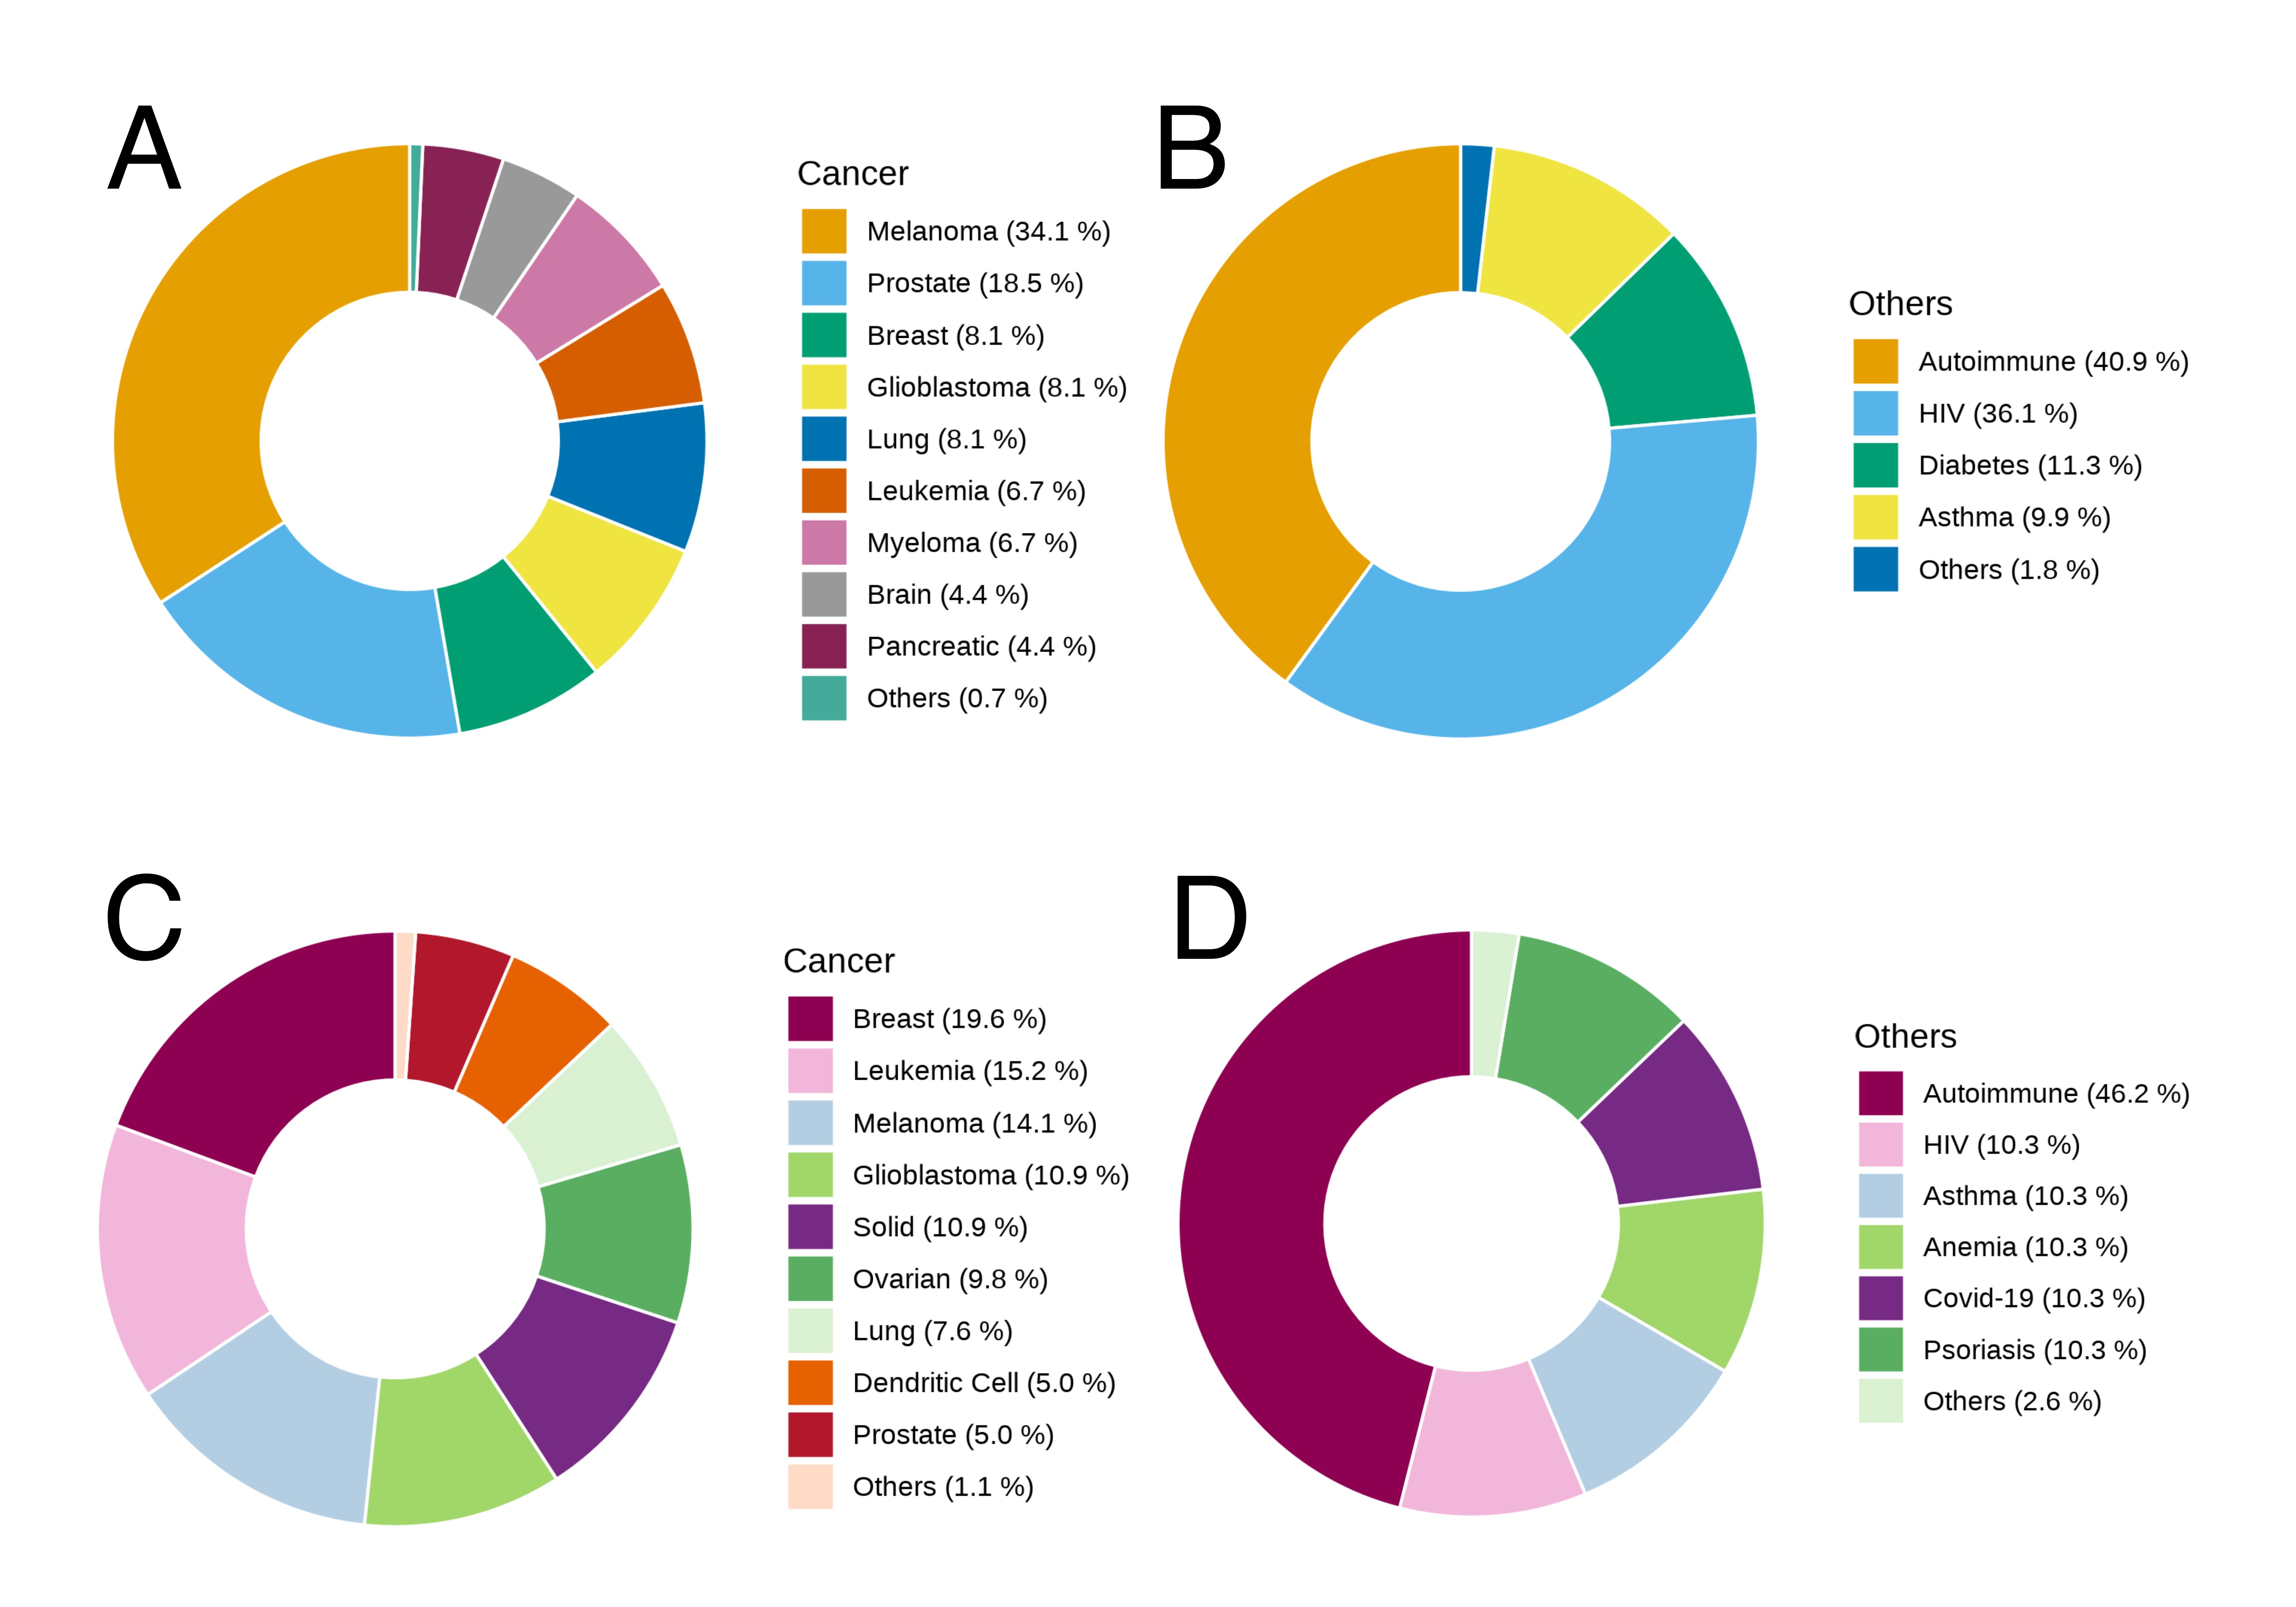
\includegraphics{images/clin_trials.png}

}

\caption{\label{fig-clin}Overview of completed (A \& B) and ongoing (C
\& D) clinical trials of dendritic cell vaccination for therapy in
cancer and other dieseases.}

\end{figure}%

\subsection{Combinatorial Therapies}\label{combinatorial-therapies}

\subsubsection{Synergy with Other Immunotherapeutic
Approaches}\label{synergy-with-other-immunotherapeutic-approaches}

Cytotoxic treatments can exert various positive effects on the immune
system, ranging from the simple release of tumor antigens due to cancer
cell lysis to more complex immunological impacts. The release of tumor
antigens enhances the uptake and presentation of a diverse array of
antigens, promoting T-cell activation. The immunological effects induced
by cytotoxic actions involve the increased expression of
immuno-stimulatory molecules (for e.g., DAMPs), heightened tumor antigen
expression, decreased proliferation of suppressor cells, and promote
proliferation and activation of cytotoxic T lymphocytes (CTLs) (35). In
a clinical example, 26 patients with different types of advanced and
treatment-refractory cancers underwent combined therapy involving
radiation, immature dendritic cells, keyhole limpet hemocyanin, and
T-cells. The initial treatment successfully eliminated metastatic and
recurrent tumors in 21 out of 26 patients, with half of them exhibiting
a complete response and no evidence of disease recurrence. These
encouraging outcomes provide impetus for further exploration of research
into combining conventional therapies with DC-based anti-tumor
immunotherapy (61). Additionally, low doses of cyclophosphamide and
paclitaxel have been demonstrated to stimulate DC maturation. As a
result, these agents are employed in combination with DC vaccines to
enhance their efficacy (63).

Tumors can create an immunosuppressive environment by expressing
negative co-stimulatory molecules and secreting factors that inhibit
both innate and adaptive immunity. This immunosuppressive milieu employs
various mechanisms to evade immune surveillance, including the loss of
tumor antigen expression, alterations in MHC molecules, induction of
Treg cells, expression of inhibitory ligands, lack of co-stimulation,
presence of indoleamine 2,3-dioxygenase promoting Treg cell generation,
and production of immunosuppressive cytokines such as IL-10, IL-6, and
TGF-β. Overcoming this tolerance and suppression within the tumor
microenvironment is crucial for enhancing the immunogenicity and
effectiveness of DC vaccines \emph{in vivo} (14).

Combining DC-based vaccines with the blockade of inhibitory signals
holds significant promise for eliciting a more robust immune response
against cancer. Disrupting the interaction between the PD-1 receptor on
activated T-cells and its ligand PD-L1 which is overexpressed on tumors
and dendritic cells showed improved \emph{in vitro} immune responses.
Strategies to interfere with this mechanism include the use of anti-PD-1
antibodies or small interfering RNA (siRNA) to silence PD-L1 and PD-L2
ligands on dendritic cells (64).

Another valuable target is the cytotoxic T lymphocyte-associated antigen
4 (CTLA-4), which inhibits T-cell activation. Blocking CTLA-4 with
antibodies, such as ipilimumab, has demonstrated therapeutic efficacy
and received FDA approval for treating metastatic melanoma in 2011 (42).

The JAK/STAT signaling pathway, which is crucial for proper dendritic
cell (DC) function, can be negatively regulated by the suppressors of
cytokine signaling (SOCS) family and glucocorticoid-induced leucine
zipper (GILZ). Targeting these inhibitory components, such as by using
siRNA to silence SOCS expression, represents a promising strategy to
enhance DC functionality and improve immune responses. By relieving the
inhibitory effects of SOCS and GILZ on JAK/STAT signaling in DCs, their
antigen presentation, cytokine production, and T-cell stimulatory
capacities may be augmented, providing additional avenues for
immunomodulation (85). Inhibiting GILZ has potential therapeutic
benefits by altering DC maturation in response to TLR agonists and
CD40L, as demonstrated in studies. Furthermore, GILZ expression in
macrophages within Burkitt lymphomas has been linked to immune system
failure to reject the tumor (66).

Immunotherapeutic strategies directed at inhibiting immuno-suppressive
cytokines like TGF-β and IL-10 are also under exploration to enhance
vaccine effectiveness. IL-10 receptor antibodies have shown promise in
enhancing specific immune responses and IL-12 production (67).
Additionally, inhibiting TGF-β has been associated with suppressing
T\textsubscript{reg} cell proliferation and increasing the number of
TAA-specific T-cells (68).

\subsubsection{Prospects for Personalized Combinatorial
Therapies}\label{prospects-for-personalized-combinatorial-therapies}

Alternative cancer immunotherapies exhibiting promise encompass cellular
transfer of tumor-infiltrating lymphocytes (TILs), genetically modified
T-cells, and antibodies targeting immune checkpoint inhibitors (86).
Adoptive cellular therapy (ACT) involves isolation and expansion of
antigen-specific T-cells \emph{ex vivo} for later transfer back to
patients (87). Despite its success in hematologic malignancies and
melanoma, ACT's efficacy against most solid tumors is limited, primarily
due to T-cells' inability to function and persist \emph{in vivo}.
Obstacles include the necessity for tumor resection, challenges in
isolating or expanding TILs adequately, and the standard lymphodepletion
procedure before transfer, causing side effects in roughly 50\% of
patients (87).

An alternative approach is genetic engineering of T-cells to express
chimeric antigen receptors (CARs), linking an antigen-binding domain to
an intracellular T-cell signaling domain (88). Prominent results have
been achieved with CAR T-cells targeting CD19 in B-cell malignancies,
albeit with significant toxicity, including cytokine-release syndrome
and neurotoxicity. In contrast, DC-based immunotherapies boast a
favorable safety profile, observed over two decades in numerous trials,
with minimal toxicity and rare severe immunotoxicity reactions (91).

DC vaccines have demonstrated tolerability, inducing only localized
reactions at injection sites and occasional systemic effects like fever
and malaise. In contrast, immune checkpoint blockade can lead to
autoimmune complications affecting various organs. CTLA4 blockade, for
instance, may disrupt the effective inhibition of autoreactive T-cells,
resulting in immune-related adverse events affecting the liver, skin,
endocrine glands, and bowel (91). In summary, immunotherapy holds
promise for improving tumor outcomes. Monoclonal antibodies (mAbs),
dendritic cell vaccines, immune checkpoint blockade, and adoptive and
genetically engineered T-cell therapy have shown encouraging results.
Future directions involve integrating several approaches with standard
chemotherapy and radiotherapy, determining optimal timing for
immunotherapy initiation, and devising strategies to maximize
effectiveness while limiting toxicity.

\subsection{Conclusion \& Future
Perspectives}\label{conclusion-future-perspectives}

Recent T-cell therapy successes have sparked interest in enhancing
antitumor T-cell immunity for cancer therapy. Dendritic cells (DCs)
stand out as the most effective antigen-presenting cells (APCs) capable
of activating naive T-cells and eliciting immune memory responses
against cancer.Despite often being dysfunctional or tolerogenic in the
tumor microenvironment (TME), a deeper understanding of the regulation
of DCs in this context holds therapeutic potential in various clinical
settings. Exploring how different dendritic cell subsets may elicit
distinct functional immune responses in cancer is a notable area of
interest. For instance, the cDC1 subset is associated with the induction
of cancer-controlling immunity and increased survival in specific cancer
types (92--95). On the other hand, monocyte-derived DCs (MoDCs) play a
fundamental role during treatment with immunogenic cell death-inducing
chemotherapy agents and radiation therapy (96--98), while cDC2s are
crucial for inducing antitumor CD4\textsuperscript{+} T-cell immunity
(43,99). Although DCs can enhance the effectiveness of established
cancer therapies, the development of efficient vaccination strategies
requires a deeper understanding of dendritic cell biology and functions.
Progress in preclinical studies encourages the exploration of DCs in
more effective therapeutic treatments through clinical trials.
Strategies to achieve this involve administration in conjunction with
neo-antigens, mobilization of endogenous DCs, and the use of stimulating
adjuvants. A more precise and refined targeting of DCs could further
enhance the efficacy of these approaches. DC vaccination approaches show
promise, especially in delaying or preventing relapse and metastasis
following debulking surgical procedures. Overall, there is a need to
gain more insights into how specific DC subsets with specialized
functions can be optimally exploited to coordinate effective immune
responses against cancer.

\subsection{References}\label{references}

\phantomsection\label{refs}
\begin{CSLReferences}{0}{1}
\bibitem[\citeproctext]{ref-chen2016dendritic}
\CSLLeftMargin{1. }%
\CSLRightInline{Chen P, Liu X, Sun Y, Zhou P, Wang Y, Zhang Y. Dendritic
cell targeted vaccines: Recent progresses and challenges. Human vaccines
\& immunotherapeutics. 2016;12(3):612--22. }

\bibitem[\citeproctext]{ref-rehman2017dendritic}
\CSLLeftMargin{2. }%
\CSLRightInline{Rehman Z, Umar S, Meng C, Ullah Z, Riaz F, Rehman S, et
al. Dendritic cell harmonised immunity to poultry pathogens; a review.
World's Poultry Science Journal. 2017;73(3):581--90. }

\bibitem[\citeproctext]{ref-steinman2012decisions}
\CSLLeftMargin{3. }%
\CSLRightInline{Steinman RM. Decisions about dendritic cells: Past,
present, and future. Annual review of immunology. 2012;30:1--22. }

\bibitem[\citeproctext]{ref-wykes2000dendritic}
\CSLLeftMargin{4. }%
\CSLRightInline{Wykes M, MacPherson G. Dendritic cell--b-cell
interaction: Dendritic cells provide b cells with CD40-independent
proliferation signals and CD40-dependent survival signals. Immunology.
2000;100(1):1--3. }

\bibitem[\citeproctext]{ref-medzhitov1997human}
\CSLLeftMargin{5. }%
\CSLRightInline{Medzhitov R, Preston-Hurlburt P, Janeway Jr CA. A human
homologue of the drosophila toll protein signals activation of adaptive
immunity. Nature. 1997;388(6640):394--7. }

\bibitem[\citeproctext]{ref-van2012optimizing}
\CSLLeftMargin{6. }%
\CSLRightInline{Van Brussel I, Berneman ZN, Cools N, et al. Optimizing
dendritic cell-based immunotherapy: Tackling the complexity of different
arms of the immune system. Mediators of inflammation. 2012;2012. }

\bibitem[\citeproctext]{ref-palucka2012cancer}
\CSLLeftMargin{7. }%
\CSLRightInline{Palucka K, Banchereau J. Cancer immunotherapy via
dendritic cells. Nature Reviews Cancer. 2012;12(4):265--77. }

\bibitem[\citeproctext]{ref-steinman2007taking}
\CSLLeftMargin{8. }%
\CSLRightInline{Steinman RM, Banchereau J. Taking dendritic cells into
medicine. Nature. 2007;449(7161):419--26. }

\bibitem[\citeproctext]{ref-borghaei2009immunotherapy}
\CSLLeftMargin{9. }%
\CSLRightInline{Borghaei H, Smith MR, Campbell KS. Immunotherapy of
cancer. European journal of pharmacology. 2009;625(1-3):41--54. }

\bibitem[\citeproctext]{ref-boudreau2011engineering}
\CSLLeftMargin{10. }%
\CSLRightInline{Boudreau JE, Bonehill A, Thielemans K, Wan Y.
Engineering dendritic cells to enhance cancer immunotherapy. Molecular
therapy. 2011;19(5):841--53. }

\bibitem[\citeproctext]{ref-joffre2012cross}
\CSLLeftMargin{11. }%
\CSLRightInline{Joffre OP, Segura E, Savina A, Amigorena S.
Cross-presentation by dendritic cells. Nature Reviews Immunology.
2012;12(8):557--69. }

\bibitem[\citeproctext]{ref-nair2012isolation}
\CSLLeftMargin{12. }%
\CSLRightInline{Nair S, Archer GE, Tedder TF. Isolation and generation
of human dendritic cells. Current protocols in immunology.
2012;99(1):7--32. }

\bibitem[\citeproctext]{ref-tedder1997isolation}
\CSLLeftMargin{13. }%
\CSLRightInline{Tedder TF, Jansen PJ. Isolation and generation of human
dendritic cells. Current protocols in immunology. 1997;23(1):7--32. }

\bibitem[\citeproctext]{ref-zhou1996cd14}
\CSLLeftMargin{14. }%
\CSLRightInline{Zhou LJ, Tedder TF. CD14+ blood monocytes can
differentiate into functionally mature CD83+ dendritic cells.
Proceedings of the National Academy of Sciences. 1996;93(6):2588--92. }

\bibitem[\citeproctext]{ref-sabado2010directing}
\CSLLeftMargin{15. }%
\CSLRightInline{Sabado RL, Bhardwaj N. Directing dendritic cell
immunotherapy towards successful cancer treatment. Immunotherapy.
2010;2(1):37--56. }

\bibitem[\citeproctext]{ref-amedei2011novel}
\CSLLeftMargin{16. }%
\CSLRightInline{Amedei A, Benagiano M, Bella C della, Niccolai E,
D'Elios MM, et al. Novel immunotherapeutic strategies of gastric cancer
treatment. BioMed Research International. 2011;2011. }

\bibitem[\citeproctext]{ref-nicolette2007dendritic}
\CSLLeftMargin{17. }%
\CSLRightInline{Nicolette C, Healey D, Tcherepanova I, Whelton P,
Monesmith T, Coombs L, et al. Dendritic cells for active immunotherapy:
Optimizing design and manufacture in order to develop commercially and
clinically viable products. Vaccine. 2007;25:B47--60. }

\bibitem[\citeproctext]{ref-fanger1996type}
\CSLLeftMargin{18. }%
\CSLRightInline{Fanger NA, Wardwell K, Shen L, Tedder TF, Guyre PM. Type
i (CD64) and type II (CD32) fc gamma receptor-mediated phagocytosis by
human blood dendritic cells. Journal of immunology (Baltimore, Md:
1950). 1996;157(2):541--8. }

\bibitem[\citeproctext]{ref-o2005generation}
\CSLLeftMargin{19. }%
\CSLRightInline{O'Neill D, Bhardwaj N. Generation of autologous
peptide-and protein-pulsed dendritic cells for patient-specific
immunotherapy. Adoptive Immunotherapy: Methods and Protocols.
2005;97--112. }

\bibitem[\citeproctext]{ref-schnurr2005tumor}
\CSLLeftMargin{20. }%
\CSLRightInline{Schnurr M, Chen Q, Shin A, Chen W, Toy T, Jenderek C, et
al. Tumor antigen processing and presentation depend critically on
dendritic cell type and the mode of antigen delivery. Blood.
2005;105(6):2465--72. }

\bibitem[\citeproctext]{ref-schroers2000transduction}
\CSLLeftMargin{21. }%
\CSLRightInline{Schroers R, Sinha I, Segall H, Schmidt-Wolf IG, Rooney
CM, Brenner MK, et al. Transduction of human PBMC-derived dendritic
cells and macrophages by an HIV-1-based lentiviral vector system.
Molecular Therapy. 2000;1(2):171--9. }

\bibitem[\citeproctext]{ref-dyall2001lentivirus}
\CSLLeftMargin{22. }%
\CSLRightInline{Dyall J, Latouche JB, Schnell S, Sadelain M.
Lentivirus-transduced human monocyte-derived dendritic cells efficiently
stimulate antigen-specific cytotoxic t lymphocytes. Blood, The Journal
of the American Society of Hematology. 2001;97(1):114--21. }

\bibitem[\citeproctext]{ref-lizee2004lentivirus}
\CSLLeftMargin{23. }%
\CSLRightInline{Lizée G, Gonzales MI, Topalian SL. Lentivirus
vector-mediated expression of tumor-associated epitopes by human antigen
presenting cells. Human gene therapy. 2004;15(4):393--404. }

\bibitem[\citeproctext]{ref-yang2008engineered}
\CSLLeftMargin{24. }%
\CSLRightInline{Yang L, Yang H, Rideout K, Cho T, Joo K il, Ziegler L,
et al. Engineered lentivector targeting of dendritic cells for in vivo
immunization. Nature biotechnology. 2008;26(3):326--34. }

\bibitem[\citeproctext]{ref-nair2002induction}
\CSLLeftMargin{25. }%
\CSLRightInline{Nair SK, Morse M, Boczkowski D, Cumming RI, Vasovic L,
Gilboa E, et al. Induction of tumor-specific cytotoxic t lymphocytes in
cancer patients by autologous tumor RNA-transfected dendritic cells.
Annals of surgery. 2002;235(4):540. }

\bibitem[\citeproctext]{ref-gilboa2004cancer}
\CSLLeftMargin{26. }%
\CSLRightInline{Gilboa E, Vieweg J. Cancer immunotherapy with
mRNA-transfected dendritic cells. Immunological reviews.
2004;199(1):251--63. }

\bibitem[\citeproctext]{ref-heiser2001human}
\CSLLeftMargin{27. }%
\CSLRightInline{Heiser A, Maurice MA, Yancey DR, Coleman DM, Dahm P,
Vieweg J. Human dendritic cells transfected with renal tumor RNA
stimulate polyclonal t-cell responses against antigens expressed by
primaryand metastatic tumors. Cancer research. 2001;61(8):3388--93. }

\bibitem[\citeproctext]{ref-doyle1987interaction}
\CSLLeftMargin{28. }%
\CSLRightInline{Doyle C, Strominger JL. Interaction between CD4 and
class II MHC molecules mediates cell adhesion. Nature.
1987;330(6145):256--9. }

\bibitem[\citeproctext]{ref-engleman1981activation}
\CSLLeftMargin{29. }%
\CSLRightInline{Engleman EG, Benike C, Grumet FC, Evans R. Activation of
human t lymphocyte subsets: Helper and suppressor/cytotoxic t cells
recognize and respond to distinct histocompatibility antigens. Journal
of immunology (Baltimore, Md: 1950). 1981;127(5):2124--9. }

\bibitem[\citeproctext]{ref-reis1993phagocytosis}
\CSLLeftMargin{30. }%
\CSLRightInline{Reis e Sousa C, Austyn JM. Phagocytosis of antigens by
langerhans cells. Dendritic Cells in Fundamental and Clinical
Immunology. 1993;199--204. }

\bibitem[\citeproctext]{ref-hoffmann2012autonomous}
\CSLLeftMargin{31. }%
\CSLRightInline{Hoffmann E, Kotsias F, Visentin G, Bruhns P, Savina A,
Amigorena S. Autonomous phagosomal degradation and antigen presentation
in dendritic cells. Proceedings of the National Academy of Sciences.
2012;109(36):14556--61. }

\bibitem[\citeproctext]{ref-garrett2000developmental}
\CSLLeftMargin{32. }%
\CSLRightInline{Garrett WS, Chen LM, Kroschewski R, Ebersold M, Turley
S, Trombetta S, et al. Developmental control of endocytosis in dendritic
cells by Cdc42. Cell. 2000;102(3):325--34. }

\bibitem[\citeproctext]{ref-platt2010mature}
\CSLLeftMargin{33. }%
\CSLRightInline{Platt CD, Ma JK, Chalouni C, Ebersold M, Bou-Reslan H,
Carano RA, et al. Mature dendritic cells use endocytic receptors to
capture and present antigens. Proceedings of the National Academy of
Sciences. 2010;107(9):4287--92. }

\bibitem[\citeproctext]{ref-bonifaz2004vivo}
\CSLLeftMargin{34. }%
\CSLRightInline{Bonifaz LC, Bonnyay DP, Charalambous A, Darguste DI,
Fujii SI, Soares H, et al. In vivo targeting of antigens to maturing
dendritic cells via the DEC-205 receptor improves t cell vaccination.
The Journal of experimental medicine. 2004;199(6):815--24. }

\bibitem[\citeproctext]{ref-sallusto1995dendritic}
\CSLLeftMargin{35. }%
\CSLRightInline{Sallusto F, Cella M, Danieli C, Lanzavecchia A.
Dendritic cells use macropinocytosis and the mannose receptor to
concentrate macromolecules in the major histocompatibility complex class
II compartment: Downregulation by cytokines and bacterial products. The
Journal of experimental medicine. 1995;182(2):389--400. }

\bibitem[\citeproctext]{ref-norbury1997constitutive}
\CSLLeftMargin{36. }%
\CSLRightInline{Norbury CC, Chambers BJ, Prescott AR, Ljunggren HG,
Watts C. Constitutive macropinocytosis allows TAP-dependent major
histocompatibility compex class i presentation of exogenous soluble
antigen by bone marrow-derived dendritic cells. European journal of
immunology. 1997;27(1):280--8. }

\bibitem[\citeproctext]{ref-niess2005cx3cr1}
\CSLLeftMargin{37. }%
\CSLRightInline{Niess JH, Brand S, Gu X, Landsman L, Jung S, McCormick
BA, et al. CX3CR1-mediated dendritic cell access to the intestinal lumen
and bacterial clearance. Science. 2005;307(5707):254--8. }

\bibitem[\citeproctext]{ref-rescigno2001dendritic}
\CSLLeftMargin{38. }%
\CSLRightInline{Rescigno M, Urbano M, Valzasina B, Francolini M, Rotta
G, Bonasio R, et al. Dendritic cells express tight junction proteins and
penetrate gut epithelial monolayers to sample bacteria. Nature
immunology. 2001;2(4):361--7. }

\bibitem[\citeproctext]{ref-tordesillas2018pdl2x}
\CSLLeftMargin{39. }%
\CSLRightInline{Tordesillas L, Lozano-Ojalvo D, Dunkin D, Mondoulet L,
Agudo J, Merad M, et al. PDL2+ CD11b+ dermal dendritic cells capture
topical antigen through hair follicles to prime LAP+ tregs. Nature
communications. 2018;9(1):5238. }

\bibitem[\citeproctext]{ref-yao2018langerhans}
\CSLLeftMargin{40. }%
\CSLRightInline{Yao C, Kaplan DH. Langerhans cells transfer targeted
antigen to dermal DC and acquire MHC-II in vivo. The Journal of
investigative dermatology. 2018;138(7):1665. }

\bibitem[\citeproctext]{ref-deckers2017epicutaneous}
\CSLLeftMargin{41. }%
\CSLRightInline{Deckers J, Sichien D, Plantinga M, Van Moorleghem J,
Vanheerswynghels M, Hoste E, et al. Epicutaneous sensitization to house
dust mite allergen requires interferon regulatory factor 4--dependent
dermal dendritic cells. Journal of Allergy and Clinical Immunology.
2017;140(5):1364--77. }

\bibitem[\citeproctext]{ref-gerner2015strategically}
\CSLLeftMargin{42. }%
\CSLRightInline{Gerner MY, Torabi-Parizi P, Germain RN. Strategically
localized dendritic cells promote rapid t cell responses to lymph-borne
particulate antigens. Immunity. 2015;42(1):172--85. }

\bibitem[\citeproctext]{ref-binnewies2019unleashing}
\CSLLeftMargin{43. }%
\CSLRightInline{Binnewies M, Mujal AM, Pollack JL, Combes AJ, Hardison
EA, Barry KC, et al. Unleashing type-2 dendritic cells to drive
protective antitumor CD4+ t cell immunity. Cell. 2019;177(3):556--71. }

\bibitem[\citeproctext]{ref-sixt2005conduit}
\CSLLeftMargin{44. }%
\CSLRightInline{Sixt M, Kanazawa N, Selg M, Samson T, Roos G, Reinhardt
DP, et al. The conduit system transports soluble antigens from the
afferent lymph to resident dendritic cells in the t cell area of the
lymph node. Immunity. 2005;22(1):19--29. }

\bibitem[\citeproctext]{ref-gretz2000lymph}
\CSLLeftMargin{45. }%
\CSLRightInline{Gretz JE, Norbury CC, Anderson AO, Proudfoot AE, Shaw S.
Lymph-borne chemokines and other low molecular weight molecules reach
high endothelial venules via specialized conduits while a functional
barrier limits access to the lymphocyte microenvironments in lymph node
cortex. The Journal of experimental medicine. 2000;192(10):1425--40. }

\bibitem[\citeproctext]{ref-gerner2017dendritic}
\CSLLeftMargin{46. }%
\CSLRightInline{Gerner MY, Casey KA, Kastenmuller W, Germain RN.
Dendritic cell and antigen dispersal landscapes regulate t cell
immunity. Journal of Experimental Medicine. 2017;214(10):3105--22. }

\bibitem[\citeproctext]{ref-gilfillan2018clec9ax}
\CSLLeftMargin{47. }%
\CSLRightInline{Gilfillan CB, Kuhn S, Baey C, Hyde EJ, Yang J, Ruedl C,
et al. Clec9A+ dendritic cells are not essential for antitumor CD8+ t
cell responses induced by poly i: C immunotherapy. The Journal of
Immunology. 2018;200(8):2978--86. }

\bibitem[\citeproctext]{ref-gutierrez2015cross}
\CSLLeftMargin{48. }%
\CSLRightInline{Gutiérrez-Martı́nez E, Planès R, Anselmi G, Reynolds M,
Menezes S, Adiko AC, et al. Cross-presentation of cell-associated
antigens by MHC class i in dendritic cell subsets. Frontiers in
immunology. 2015;6:363. }

\bibitem[\citeproctext]{ref-dudziak2007differential}
\CSLLeftMargin{49. }%
\CSLRightInline{Dudziak D, Kamphorst AO, Heidkamp GF, Buchholz VR,
Trumpfheller C, Yamazaki S, et al. Differential antigen processing by
dendritic cell subsets in vivo. Science. 2007;315(5808):107--11. }

\bibitem[\citeproctext]{ref-lehmann2017dc}
\CSLLeftMargin{50. }%
\CSLRightInline{Lehmann CH, Baranska A, Heidkamp GF, Heger L, Neubert K,
Lühr JJ, et al. DC subset--specific induction of t cell responses upon
antigen uptake via fc\(\gamma\) receptors in vivo. Journal of
Experimental Medicine. 2017;214(5):1509--28. }

\bibitem[\citeproctext]{ref-caminschi2008dendritic}
\CSLLeftMargin{51. }%
\CSLRightInline{Caminschi I, Proietto AI, Ahmet F, Kitsoulis S, Shin Teh
J, Lo JC, et al. The dendritic cell subtype-restricted c-type lectin
Clec9A is a target for vaccine enhancement. Blood, The Journal of the
American Society of Hematology. 2008;112(8):3264--73. }

\bibitem[\citeproctext]{ref-den2002constitutive}
\CSLLeftMargin{52. }%
\CSLRightInline{Haan JM den, Bevan MJ. Constitutive versus
activation-dependent cross-presentation of immune complexes by CD8+ and
CD8- dendritic cells in vivo. The Journal of experimental medicine.
2002;196(6):817--27. }

\bibitem[\citeproctext]{ref-ballesteros2010temporal}
\CSLLeftMargin{53. }%
\CSLRightInline{Ballesteros-Tato A, León B, Lund FE, Randall TD.
Temporal changes in dendritic cell subsets, cross-priming and
costimulation via CD70 control CD8+ t cell responses to influenza.
Nature immunology. 2010;11(3):216--24. }

\bibitem[\citeproctext]{ref-baker2011neonatal}
\CSLLeftMargin{54. }%
\CSLRightInline{Baker K, Qiao SW, Kuo TT, Aveson VG, Platzer B, Andersen
JT, et al. Neonatal fc receptor for IgG (FcRn) regulates
cross-presentation of IgG immune complexes by CD8- CD11b+ dendritic
cells. Proceedings of the National Academy of Sciences.
2011;108(24):9927--32. }

\bibitem[\citeproctext]{ref-vander2014transcriptional}
\CSLLeftMargin{55. }%
\CSLRightInline{Vander Lugt B, Khan AA, Hackney JA, Agrawal S, Lesch J,
Zhou M, et al. Transcriptional programming of dendritic cells for
enhanced MHC class II antigen presentation. Nature immunology.
2014;15(2):161--7. }

\bibitem[\citeproctext]{ref-van2016tcr}
\CSLLeftMargin{56. }%
\CSLRightInline{Van Panhuys N. TCR signal strength alters t--DC
activation and interaction times and directs the outcome of
differentiation. Frontiers in immunology. 2016;7:6. }

\bibitem[\citeproctext]{ref-mclellan2002anatomic}
\CSLLeftMargin{57. }%
\CSLRightInline{McLellan AD, Kapp M, Eggert A, Linden C, Bommhardt U,
Bröcker EB, et al. Anatomic location and t-cell stimulatory functions of
mouse dendritic cell subsets defined by CD4 and CD8 expression. Blood,
The Journal of the American Society of Hematology. 2002;99(6):2084--93.
}

\bibitem[\citeproctext]{ref-vremec2000cd4}
\CSLLeftMargin{58. }%
\CSLRightInline{Vremec D, Pooley J, Hochrein H, Wu L, Shortman K. CD4
and CD8 expression by dendritic cell subtypes in mouse thymus and
spleen. The Journal of Immunology. 2000;164(6):2978--86. }

\bibitem[\citeproctext]{ref-takeda2003toll}
\CSLLeftMargin{59. }%
\CSLRightInline{Takeda K, Kaisho T, Akira S. Toll-like receptors. Annual
review of immunology. 2003;21(1):335--76. }

\bibitem[\citeproctext]{ref-edwards2003toll}
\CSLLeftMargin{60. }%
\CSLRightInline{Edwards AD, Diebold SS, Slack EM, Tomizawa H, Hemmi H,
Kaisho T, et al. Toll-like receptor expression in murine DC subsets:
Lack of TLR7 expression by CD8\(\alpha\)+ DC correlates with
unresponsiveness to imidazoquinolines. European journal of immunology.
2003;33(4):827--33. }

\bibitem[\citeproctext]{ref-boonstra2003flexibility}
\CSLLeftMargin{61. }%
\CSLRightInline{Boonstra A, Asselin-Paturel C, Gilliet M, Crain C,
Trinchieri G, Liu YJ, et al. Flexibility of mouse classical and
plasmacytoid-derived dendritic cells in directing t helper type 1 and 2
cell development: Dependency on antigen dose and differential toll-like
receptor ligation. The Journal of experimental medicine.
2003;197(1):101--9. }

\bibitem[\citeproctext]{ref-boonstra2006macrophages}
\CSLLeftMargin{62. }%
\CSLRightInline{Boonstra A, Rajsbaum R, Holman M, Marques R,
Asselin-Paturel C, Pereira JP, et al. Macrophages and myeloid dendritic
cells, but not plasmacytoid dendritic cells, produce IL-10 in response
to MyD88-and TRIF-dependent TLR signals, and TLR-independent signals.
The Journal of Immunology. 2006;177(11):7551--8. }

\bibitem[\citeproctext]{ref-shortman2009improving}
\CSLLeftMargin{63. }%
\CSLRightInline{Shortman K, Lahoud MH, Caminschi I. Improving vaccines
by targeting antigens to dendritic cells. Experimental \& molecular
medicine. 2009;41(2):61--6. }

\bibitem[\citeproctext]{ref-tacken2006targeting}
\CSLLeftMargin{64. }%
\CSLRightInline{Tacken PJ, Torensma R, Figdor CG. Targeting antigens to
dendritic cells in vivo. Immunobiology. 2006;211(6-8):599--608. }

\bibitem[\citeproctext]{ref-jinushi2009cytokine}
\CSLLeftMargin{65. }%
\CSLRightInline{Jinushi M, Tahara H. Cytokine gene-mediated
immunotherapy: Current status and future perspectives. Cancer science.
2009;100(8):1389--96. }

\bibitem[\citeproctext]{ref-luiten2005immunogenicity}
\CSLLeftMargin{66. }%
\CSLRightInline{Luiten RM, Kueter EW, Mooi W, Gallee MP, Rankin EM,
Gerritsen WR, et al. Immunogenicity, including vitiligo, and feasibility
of vaccination with autologous GM-CSF--transduced tumor cells in
metastatic melanoma patients. Journal of clinical oncology.
2005;23(35):8978--91. }

\bibitem[\citeproctext]{ref-small2007granulocyte}
\CSLLeftMargin{67. }%
\CSLRightInline{Small EJ, Sacks N, Nemunaitis J, Urba WJ, Dula E,
Centeno AS, et al. Granulocyte macrophage colony-stimulating
factor--secreting allogeneic cellular immunotherapy for
hormone-refractory prostate cancer. Clinical Cancer Research.
2007;13(13):3883--91. }

\bibitem[\citeproctext]{ref-higano2008phase}
\CSLLeftMargin{68. }%
\CSLRightInline{Higano CS, Corman JM, Smith DC, Centeno AS, Steidle CP,
Gittleman M, et al. Phase 1/2 dose-escalation study of a
GM-CSF-secreting, allogeneic, cellular immunotherapy for metastatic
hormone-refractory prostate cancer. Cancer. 2008;113(5):975--84. }

\bibitem[\citeproctext]{ref-filipazzi2007identification}
\CSLLeftMargin{69. }%
\CSLRightInline{Filipazzi P, Valenti R, Huber V, Pilla L, Canese P, Iero
M, et al. Identification of a new subset of myeloid suppressor cells in
peripheral blood of melanoma patients with modulation by a
granulocyte-macrophage colony-stimulation factor--based antitumor
vaccine. Journal of clinical oncology. 2007;25(18):2546--53. }

\bibitem[\citeproctext]{ref-sica2007altered}
\CSLLeftMargin{70. }%
\CSLRightInline{Sica A, Bronte V, et al. Altered macrophage
differentiation and immune dysfunction in tumor development. The Journal
of clinical investigation. 2007;117(5):1155--66. }

\bibitem[\citeproctext]{ref-carter2006preferential}
\CSLLeftMargin{71. }%
\CSLRightInline{Carter RW, Thompson C, Reid DM, Wong SY, Tough DF.
Preferential induction of CD4+ t cell responses through in vivo
targeting of antigen to dendritic cell-associated c-type lectin-1. The
Journal of Immunology. 2006;177(4):2276--84. }

\bibitem[\citeproctext]{ref-boscardin2006antigen}
\CSLLeftMargin{72. }%
\CSLRightInline{Boscardin SB, Hafalla JC, Masilamani RF, Kamphorst AO,
Zebroski HA, Rai U, et al. Antigen targeting to dendritic cells elicits
long-lived t cell help for antibody responses. The Journal of
experimental medicine. 2006;203(3):599--606. }

\bibitem[\citeproctext]{ref-ramakrishna2004mannose}
\CSLLeftMargin{73. }%
\CSLRightInline{Ramakrishna V, Treml JF, Vitale L, Connolly JE, O'Neill
T, Smith PA, et al. Mannose receptor targeting of tumor antigen pmel17
to human dendritic cells directs anti-melanoma t cell responses via
multiple HLA molecules. The Journal of Immunology. 2004;172(5):2845--52.
}

\bibitem[\citeproctext]{ref-tacken2005effective}
\CSLLeftMargin{74. }%
\CSLRightInline{Tacken PJ, Vries IJM de, Gijzen K, Joosten B, Wu D,
Rother RP, et al. Effective induction of naive and recall t-cell
responses by targeting antigen to human dendritic cells via a humanized
anti--DC-SIGN antibody. Blood. 2005;106(4):1278--85. }

\bibitem[\citeproctext]{ref-hodge2000enhanced}
\CSLLeftMargin{75. }%
\CSLRightInline{Hodge JW, Rad AN, Grosenbach DW, Sabzevari H, Yafal AG,
Gritz L, et al. Enhanced activation of t cells by dendritic cells
engineered to hyperexpress a triad of costimulatory molecules. Journal
of the National Cancer Institute. 2000;92(15):1228--39. }

\bibitem[\citeproctext]{ref-steinman2002avoiding}
\CSLLeftMargin{76. }%
\CSLRightInline{Steinman RM, Nussenzweig MC. Avoiding horror
autotoxicus: The importance of dendritic cells in peripheral t cell
tolerance. Proceedings of the National Academy of Sciences.
2002;99(1):351--8. }

\bibitem[\citeproctext]{ref-de2003maturation}
\CSLLeftMargin{77. }%
\CSLRightInline{Vries IJM de, Lesterhuis WJ, Scharenborg NM, Engelen LP,
Ruiter DJ, Gerritsen MJP, et al. Maturation of dendritic cells is a
prerequisite for inducing immune responses in advanced melanoma
patients. Clinical cancer research. 2003;9(14):5091--100. }

\bibitem[\citeproctext]{ref-jonuleit2001comparison}
\CSLLeftMargin{78. }%
\CSLRightInline{Jonuleit H, Giesecke-Tuettenberg A, Tüting T,
Thurner-Schuler B, Stuge TB, Paragnik L, et al. A comparison of two
types of dendritic cell as adjuvants for the induction of
melanoma-specific t-cell responses in humans following intranodal
injection. International journal of cancer. 2001;93(2):243--51. }

\bibitem[\citeproctext]{ref-mastelic2019personalized}
\CSLLeftMargin{79. }%
\CSLRightInline{Mastelic-Gavillet B, Balint K, Boudousquie C, Gannon PO,
Kandalaft LE. Personalized dendritic cell vaccines---recent
breakthroughs and encouraging clinical results. Frontiers in immunology.
2019;10:766. }

\bibitem[\citeproctext]{ref-laureano2022trial}
\CSLLeftMargin{80. }%
\CSLRightInline{Laureano RS VI Sprooten J. Trial watch: Dendritic cell
(DC)-based immunotherapy for cancer. Oncoimmunology. 2022;1(1). }

\bibitem[\citeproctext]{ref-europeancommission2003}
\CSLLeftMargin{81. }%
\CSLRightInline{Commission E. Commission directive 2003/63/EC of 25 june
2003 amending directive 2001/83/EC of the european parliament and of the
council on the community code relating to medicinal products for human
use (text with EEA relevance). European Commission. }

\bibitem[\citeproctext]{ref-steinman1997-mc}
\CSLLeftMargin{82. }%
\CSLRightInline{Steinman RM, Pack M, Inaba K. Dendritic cell development
and maturation. Adv Exp Med Biol. 1997;417:1--6. }

\bibitem[\citeproctext]{ref-mellman2001-gu}
\CSLLeftMargin{83. }%
\CSLRightInline{Mellman I, Steinman RM. Dendritic cells: Specialized and
regulated antigen processing machines. Cell. 2001 Aug;106(3):255--8. }

\bibitem[\citeproctext]{ref-sabado2016-be}
\CSLLeftMargin{84. }%
\CSLRightInline{Sabado RL, Meseck M, Bhardwaj N. Dendritic cell
vaccines. Methods Mol Biol. 2016;1403:763--77. }

\bibitem[\citeproctext]{ref-jinushi2008enhancing}
\CSLLeftMargin{85. }%
\CSLRightInline{Jinushi M, Hodi FS, Dranoff G. Enhancing the clinical
activity of granulocyte-macrophage colony-stimulating factor-secreting
tumor cell vaccines. Immunological reviews. 2008;222(1):287--98. }

\bibitem[\citeproctext]{ref-abbott2019-ll}
\CSLLeftMargin{86. }%
\CSLRightInline{Abbott M, Ustoyev Y. Cancer and the immune system: The
history and background of immunotherapy. Semin Oncol Nurs. 2019
Oct;35(5):150923. }

\bibitem[\citeproctext]{ref-chan2021-vo}
\CSLLeftMargin{87. }%
\CSLRightInline{Chan JD, Lai J, Slaney CY, Kallies A, Beavis PA, Darcy
PK. Cellular networks controlling {T} cell persistence in adoptive cell
therapy. Nat Rev Immunol. 2021 Dec;21(12):769--84. }

\bibitem[\citeproctext]{ref-guo2021-fo}
\CSLLeftMargin{88. }%
\CSLRightInline{Guo J, Kent A, Davila E. Chimeric non-antigen receptors
in {T} cell-based cancer therapy. J Immunother Cancer. 2021
Aug;9(8):e002628. }

\bibitem[\citeproctext]{ref-perez2019-gb}
\CSLLeftMargin{89. }%
\CSLRightInline{Perez CR, De Palma M. Engineering dendritic cell
vaccines to improve cancer immunotherapy. Nat Commun. 2019
Nov;10(1):5408. }

\bibitem[\citeproctext]{ref-kang2022-fo}
\CSLLeftMargin{90. }%
\CSLRightInline{Kang BH, Lee HK. Dendritic cell-based immunotherapy in
hot and cold tumors. Int J Mol Sci. 2022 Jun;23(13):7325. }

\bibitem[\citeproctext]{ref-sabado2017-zn}
\CSLLeftMargin{91. }%
\CSLRightInline{Sabado RL, Balan S, Bhardwaj N. Dendritic cell-based
immunotherapy. Cell Res. 2017 Jan;27(1):74--95. }

\bibitem[\citeproctext]{ref-salmon2016expansion}
\CSLLeftMargin{92. }%
\CSLRightInline{Salmon H, Idoyaga J, Rahman A, Leboeuf M, Remark R,
Jordan S, et al. Expansion and activation of CD103+ dendritic cell
progenitors at the tumor site enhances tumor responses to therapeutic
PD-L1 and BRAF inhibition. Immunity. 2016;44(4):924--38. }

\bibitem[\citeproctext]{ref-sanchez2016cancer}
\CSLLeftMargin{93. }%
\CSLRightInline{Sánchez-Paulete AR, Cueto FJ, Martı́nez-López M, Labiano
S, Morales-Kastresana A, Rodrı́guez-Ruiz ME, et al. Cancer immunotherapy
with immunomodulatory anti-CD137 and anti--PD-1 monoclonal antibodies
requires BATF3-dependent dendritic cells. Cancer discovery.
2016;6(1):71--9. }

\bibitem[\citeproctext]{ref-wculek2019effective}
\CSLLeftMargin{94. }%
\CSLRightInline{Wculek SK, Amores-Iniesta J, Conde-Garrosa R, Khouili
SC, Melero I, Sancho D. Effective cancer immunotherapy by natural mouse
conventional type-1 dendritic cells bearing dead tumor antigen. Journal
for immunotherapy of cancer. 2019;7:1--16. }

\bibitem[\citeproctext]{ref-theisen2018wdfy4}
\CSLLeftMargin{95. }%
\CSLRightInline{Theisen DJ, Davidson IV JT, Briseño CG, Gargaro M,
Lauron EJ, Wang Q, et al. WDFY4 is required for cross-presentation in
response to viral and tumor antigens. Science. 2018;362(6415):694--9. }

\bibitem[\citeproctext]{ref-ma2013anticancer}
\CSLLeftMargin{96. }%
\CSLRightInline{Ma Y, Adjemian S, Mattarollo SR, Yamazaki T, Aymeric L,
Yang H, et al. Anticancer chemotherapy-induced intratumoral recruitment
and differentiation of antigen-presenting cells. Immunity.
2013;38(4):729--41. }

\bibitem[\citeproctext]{ref-casares2005caspase}
\CSLLeftMargin{97. }%
\CSLRightInline{Casares N, Pequignot MO, Tesniere A, Ghiringhelli F,
Roux S, Chaput N, et al. Caspase-dependent immunogenicity of
doxorubicin-induced tumor cell death. The Journal of experimental
medicine. 2005;202(12):1691--701. }

\bibitem[\citeproctext]{ref-apetoh2007toll}
\CSLLeftMargin{98. }%
\CSLRightInline{Apetoh L, Ghiringhelli F, Tesniere A, Obeid M, Ortiz C,
Criollo A, et al. Toll-like receptor 4--dependent contribution of the
immune system to anticancer chemotherapy and radiotherapy. Nature
medicine. 2007;13(9):1050--9. }

\bibitem[\citeproctext]{ref-laoui2016tumour}
\CSLLeftMargin{99. }%
\CSLRightInline{Laoui D, Keirsse J, Morias Y, Van Overmeire E, Geeraerts
X, Elkrim Y, et al. The tumour microenvironment harbours ontogenically
distinct dendritic cell populations with opposing effects on tumour
immunity. Nature communications. 2016;7(1):13720. }

\end{CSLReferences}



\end{document}
